\documentclass[groupedaddress,rmp,amsmath,amssymb,bibnotes,altaffilletter,twocolumn]{revtex4-1}

%Please change this with your Unidoc number!
\newcommand{\docno}{yyyy-nnn}

\usepackage{lineno}
\usepackage{longtable}  
\usepackage{url}
\usepackage{hyperref}
\usepackage{graphicx}
\usepackage{amsmath,amssymb,bbold,bm}
\usepackage{epstopdf}
\usepackage{xcolor}
\usepackage{lipsum}
\usepackage{gensymb}
\definecolor{blue}{RGB}{50,0,255}
\definecolor{orange}{RGB}{255,128,0}ls 	
\colorlet{blueh}{blue!30}
\usepackage{fancyhdr}
\usepackage{afterpage}
\usepackage{siunitx}
\usepackage{booktabs}
\usepackage{subcaption}
\usepackage{physics}

\fancypagestyle{uniheader}
{
\fancyhf{}% Clear all headers/footers
\fancyhead[L]{Unidoc \#M-TECHDOCUNI-\docno}% Header Centred
  \fancyfoot[C]{-\thepage-}% Footer Centred
  \renewcommand{\headrulewidth}{2pt}% 
  \renewcommand{\headheight}{52pt}% 
  \renewcommand{\headrule}{\hbox to\headwidth{%
    \color{orange}\leaders\hrule height \headrulewidth\hfill}}
  \renewcommand{\footrulewidth}{0pt}% No footer rule
  \rhead{\includegraphics[width=1cm]{figs/MJD}}
}

\usepackage{soul}
\sisetup{output-exponent-marker=\ensuremath{\mathrm{e}}}
\newcommand{\hlc}[2][yellow]{ {\sethlcolor{#1} \hl{#2}} }

\begin{document}

\def\nuc#1#2{${}^{#1}$#2}
\def\mee{$\langle m_{\beta\beta} \rangle$}
\def\mnu{$m_{\nu}$}
\def\ml{$m_{lightest}$}
\def\gnu{$\langle g_{\nu,\chi}\rangle$}
\def\mmod{$\| \langle m_{\beta\beta} \rangle \|$}
\def\mb{$\langle m_{\beta} \rangle$}
\def\BBz{$\beta\beta(0\nu)$}
\def\BBm{$\beta\beta(0\nu,\chi)$}
\def\BBt{$\beta\beta(2\nu)$}
\def\nonubb{$\beta\beta(0\nu)$}
\def\twonubb{$\beta\beta(2\nu)$}
\def\BB{$\beta\beta$}
\def\Mz{$M_{0\nu}$}
\def\Mt{$M_{2\nu}$}
\def\MzG{$M^{GT}_{0\nu}$}           %Gamov-Teller
\def\MzF{$M^{F}_{0\nu}$}                %Fermi
\def\MtG{$M^{GT}_{2\nu}$}           %Gamov-Teller
\def\MtF{$M^{F}_{2\nu}$}                %Fermi
\def\Gz{$G_{0\nu}$}					%phase space factor for 0nu
\def\Tz{$T^{0\nu}_{1/2}$}
\def\Tt{$T^{2\nu}_{1/2}$}
\def\Tc{$T^{0\nu\,\chi}_{1/2}$}
\def\Rz{$\Gamma_{0\nu}$}            %0 nu decay rate
\def\Rt{$\Gamma_{2\nu}$}            %2 nu decay rateq
\def\ms{$\delta m_{\rm sol}^{2}$}
\def\ma{$\delta m_{\rm atm}^{2}$}
\def\mot{$\delta m_{12}^{2}$}
\def\mtt{$\delta m_{23}^{2}$}
\def\ts{$\theta_{\rm sol}$}
\def\ta{$\theta_{\rm atm}$}
\def\ttwo{$\theta_{12}$}
\def\tot{$\theta_{13}$}
\def\gpp{$g_{pp}$}                  % the g_pp of QRPA fame
\def\gA{$g_{A}$}                  % the Axial Vector coupling constant
\def\qval{$Q_{\beta\beta}$}                 % The Q-value
\def\be{\begin{equation}}
\def\ee{\end{equation}}
\def\cpKkgy{cnts/(keV kg y)}
\def\cpKkgd{cnts/(keV kg d)}
\def\cpRty{cnts/(ROI t y)}
\def\onecpRty{1~cnt/(ROI t y)}
\def\threecpRty{3~cnts/(ROI t y)}
\def\ppc{P-PC}                          % P-type Point Contact
\def\nsc{N-SC}                          % N-type Segmented Contact
\def\cosixty{$^{60}Co$}
\def\thttt{$^{232}\mathrm{Th}$}
\def\thtte{$^{228}\mathrm{Th}$}
\def\utte{$^{238}\mathrm{U}$}
\def\am{$^{241}\mathrm{Am}$}
\def\po{$^{210}\mathrm{Po}$}
\def\mubqkg{$\mu\mathrm{Bq/kg}$}
\def\cusulfate{$\mathrm{CuSO}_4$}
\def\MJ{{\sc Majorana}}             %Majorana project name
\def\DEM{{\sc Demonstrator}}             %Demonstrator in small caps
\def\MJDEMbf{\bfseries{\scshape{Majorana Demonstrator}}}
\def\MJbf{\bfseries{\scshape{Majorana}}}
\def\MJDEMit{\itshape{\scshape{Majorana Demonstrator}}}
\newcommand{\Gerda}{GERDA}
\newcommand{\GF}{\textsc{Geant4}}
\newcommand{\MaGe}{\textsc{MaGe}}


\newcommand{\bhsu}{Black Hills State University, Spearfish, SD, USA}
\newcommand{\duke}{Duke University, Durham, NC, USA}
\newcommand{\kurchatov}{National Research Center “Kurchatov Institute” Institute for Theoretical and Experimental Physics, Moscow, Russia}
\newcommand{\jinr}{Joint Institute for Nuclear Research, Dubna, Russia}
\newcommand{\lanl}{Los Alamos National Laboratory, Los Alamos, NM, USA}
\newcommand{\lbnl}{Lawrence Berkeley National Laboratory, Berkeley, CA ,USA}
\newcommand{\ncsu}{North Carolina State University, Raleigh, NC, USA}
\newcommand{\ornl}{Oak Ridge National Laboratory, Oak Ridge, TN, USA}
\newcommand{\rcnp}{Research Center for Nuclear Physics, Osaka University, Ibaraki, Japan}
\newcommand{\pnnl}{Pacific Northwest National Laboratory, Richland, WA, USA}
\newcommand{\queens}{Queen’s University, Kingston, ON, Canada}
\newcommand{\sdsmt}{South Dakota School of Mines and Technology, Rapid City, SD, USA}
\newcommand{\tunl}{Triangle Universities Nuclear Laboratory, Durham, NC, USA}
\newcommand{\ttu}{Tennessee Tech University, Cookeville, TN, USA}
\newcommand{\unc}{University of North Carolina at Chapel Hill, Chapel Hill, NC, USA}
\newcommand{\usc}{University of South Carolina, Columbia, SC, USA}
\newcommand{\usd}{University of South Dakota, Vermillion, SD, USA}
\newcommand{\utk}{University of Tennessee, Knoxville, TN, USA}
\newcommand{\cenpa}{Center for Experimental Nuclear Physics and Astrophysics, University of Washington, Seattle, WA, USA}
\newcommand{\ucBerk}{University of California, Berkeley, USA}

%Update your title, name and affiliation
\title{Validating the DCR Effect in a \MJ\ Ortec \ppc Detector}
%These have to be in order in which they appear for the authors:
\affiliation{\cenpa}

\author{J.~Gruszko}\affiliation{\cenpa}


%%%%%% Replace the abstract here %%%%%%
\begin{abstract}
A collimated \am\ source was used to take passivated-surface scans of PONaMA-1 in the TUBE cryostat. Using these scans, the delayed-charge recovery (DCR) discriminator (see DCR unidoc) is found to effectively distinguish surface $\alpha$ interactions from bulk events at a range of event energies, including at the \nonubb\ region-of-interest. The $\alpha$-rejection efficiency of the DCR discriminator, event energy, and rate of delayed-charge recovery are studied as a function of $\alpha$ beam incidence radius (along the passivated-surface of the detector), and compared to several possible models of charge loss/delay in these events. The DCR analysis technique is shown to be complementary to fast rise-time-based $\alpha$ event discrimination (in this case, an tag based on higher-than-usual A vs. E). The overall efficiency of the DCR analysis is estimated for two models of $\alpha$ progenitor distribution on the passivated surface. The projected energy spectrum of $\alpha$ events from \po\ contamination, before and after the DCR cut, is estimated under both models of contamination.

\end{abstract}

%%%%%% Formatting, don't change these %%%%%%
\pagestyle{uniheader}

\date{\today}
\maketitle
\thispagestyle{uniheader}
\tableofcontents
%%%%%%%%%%%%

\section{Introduction}
As discussed in the DCR unidoc (reference?), $\alpha$ particle backgrounds originating on or near the passivated surface of \ppc\ detectors are a major contributor to the \MJ\ \DEM\ background spectrum, but can be identified effectively via a delayed-charge recovery (DCR) pulse-shape discriminator. While \thtte\ source calibrations and \twonubb\ events can be used to estimate the DCR acceptance of bulk events, a sample of known passivated-surface $\alpha$ events are needed to estimate the $\alpha$ rejection efficiency of the analysis. Such measurements can also be used to estimate the $\alpha$ background spectral shape both before and after the DCR cut, allowing the construction of an accurate background model for the \DEM. 

Given that the weighting potential near the passivated surface varies greatly with radius (see Fig.~\ref{fig:wp_z0}), the energy lost to delayed charge in these events, and therefore the reconstructed energy of the events, is also expected to vary with radius. Similarly, the rate of charge re-release and amount of charge released, which combine to produce the DCR parameter value, are also expected to vary with radius. These variations lead to an radially- (and therefore energy-) dependent $\alpha$ rejection efficiency. The form of the DCR and energy variation depends on the mechanism of charge delay and/or loss, including whether only electrons or both holes and electrons are affected, and whether surface-charge transport or charge-trapping (followed by re-release into the bulk) near the passivated surface is primarily responsible for the observed delayed-charge effect. 

To study these effects, a collimated \am\ source was used to scan PONaMA-1, a \ppc\ detector with the same geometry as the enriched detectors currently operating in the \MJ\ \DEM. Data was taken at with the source incident at positions spanning nearly the entire diameter of the passivated surface. 

\section{Experimental Setup}
\subsection{PONaMa-1}
The detector chosen to be scanned was PONaMA-1 (serial number TP42486A), a test-run detector produced by ORTEC using natural-abundance germanium. Its production process was identical to that used for the enriched detectors in the \DEM, and its geometry is similar to that of those detectors. Its properties are given in Table~\ref{tab:PONaMA_specs}. 

\begin{table}[]
\begin{tabular}{p{4cm} | l}
\hline
\multicolumn{2}{c}{PONaMA-1 Properties} \\
\hline
Diameter & 68.9\,mm \\ 
Height & 52.0\,mm \\ 
Dimple Diameter & 3.2\,mm \\
Dimple Depth & 2.0\,mm \\
Capacitance & 1.8\,pF \\
Depletion Voltage & 1850\,V \\
Leakage Current & 10\,pA \\
Resolution at 1332\,keV \newline (Measured at ORTEC) & 1.99\,keV \\
\end{tabular}
 \label{tab:PONaMA_specs}
\end{table}

\begin{figure*}[p]
 \centering
 \includegraphics[width=.8\textwidth]{figs/TUBE_assembly_side}
 \caption{A simplified bisected view of the TUBE scanner, showing key dimensions. The thermal braids connecting the IR umbrella to the IR cup and the mylar covering of the IR umbrella are not shown. Details of the detector cup, front-end electronics, and cold-finger are also removed for clarity.} 
 \label{fig:TUBE_side}
\end{figure*}

\subsection{The TUBE Scanner}
The TUM (Technical University of Munich) Upside-down BEGe (TUBE) scanner is a custom-built cryostat first made to study the backgrounds in GERDA due to surface interactions on the p+ electrode and groove of Canberra BEGe \ppc\ detectors. It allows a \ppc\ detector to be installed ``upside-down," with the passivated surface facing upwards, so that the surface may be scanned with a collimated source. The scanner consists of three main parts, seen in Fig.~\ref{fig:TUBE_side}: the cryostat, detector holder, and collimator assembly. 

The cryostat is made from a stainless steel tube with top and bottom flanges, with a vacuum feed-through that allows the cryostat cold-finger and signal electronics (from a Canberra vendor cryostat) to be inserted. A rail system is mounted at the top of the vessel, with a rotational feedthrough on the sidewall that allows the collimator radial position to be changed while the system is under vacuum. The collimator assembly is mounted to the carriage of this rail system, which has a pitch corresponding to 1.5\,mm of travel for every turn of the spindle. Ultra-high vacuum in the vessel is achieved using a turbomolecular pumping stand with a diaphragm forepump, connected to the system by Viton-sealed flanges. The measurements described here were taken with the pump in continuous operation, though the cooled system can retain pressures of around 1E-5\,mbar even after eight hours without pumping. 

The detector is mounted in a modified version of the original TUBE copper holder, adapted for the dimensions of PONaMA-1 by the addition of teflon shims. This holder was made by adapting the vendor-cryostat detector mount, and houses the front-end electronics. Contact with the p+ electrode is made via a spring-loaded contact pin, held in a narrow teflon holder that also provides routing for the signal cable, which runs from the contact pin to the front-end electronics. This holder creates a 6-mm ``blind spot" on the detector surface that cannot be scanned. See Fig.~\ref{fig:scan_coords}. 

This assembly is housed inside a copper IR-shield (called the ``IR cup") with a 3\,mm slit running along its diameter. This slit defines the axis that is scanned along, as the source beam shines through it onto the detector surface. See Fig.~\ref{fig:TUBE_top}. 

Further IR-shielding, required due to the high IR-shine susceptibility of the large passivated surface of ORTEC \ppc\ detectors, was added for use with PONaMA-1. It is provided by a copper ``IR umbrella" shield, mounted on the tip of the collimator and moving along with the source. This shield, which minimizes the IR-shine onto the passivated surface through the slit of the IR cup, is thermally grounded to the IR cup via two flexible high-thermal-conductivity copper braids. The dimensions of the IR umbrella were subject to the existing constraint of the TUBE cryostat chamber diameter; therefore, it does not completely cover the IR cup slit at all scanning positions. This leads to variation in the detector leakage current as the collimator is moved along the surface. The top face of the IR umbrella is covered with several layers of insulator-backed mylar, to minimize its radiative heat-load. The IR umbrella and mylar sheets have a 3\,mm diameter hole to allow the source beam to penetrate. 

\begin{figure}[h]
 \centering
 \includegraphics[width=1.0\columnwidth]{figs/TUBE_assembly_top}
 \caption{A simplified top view of the TUBE scanner, showing key dimensions.} 
 \label{fig:TUBE_top}
\end{figure}

\begin{figure}[]
 \centering
 \includegraphics[width=1.0\columnwidth]{figs/coord_system}
 \caption{A diagram showing the accessible scanning regions and the coordinate systems used to describe the source position. The dark gray and light gray regions represent the passivated surface and edge of the n+ contact surface, respectively. The gold triangle represents the source beam, which forms a $66\degree$ angle to the negative r axis. The blue region represents the portion of the detector visible through the IR cup slit, and the red region is the path traced out by the source beam. Notice that due to the misalignment of the two axes, only the region of their overlap can be scanned. The black region is the inaccessible ``blind spot" due to the contact-pin holder. It occludes all but one edge of the p+ contact region, which spans the region from $r_d = -1.6$\,mm to $r_d = 1.6$\,mm. Dimensions not to scale.} 
 \label{fig:scan_coords}
\end{figure}


\subsection{\am\ Source and Collimator Properties}

The collimator has an overall length of 53\,mm, and is suspended from the carriage of the rail system. The source is housed in a copper holder with a 1\,mm diameter collimating hole. The beam then passes through a teflon and aluminum tube, with a collimating hole of 3\,mm in diameter, that thermally isolates the source holder, carriage, and rail system from the IR umbrella. The collimator assembly ends in a copper tip with a 1\,mm diameter collimator hole, which is chamfered to create a source-beam incidence angle of $66.8\degree$ to the horizontal plane. In the course of mounting the collimator to the rail system, this angle may change by up to $2.3\degree$ in either direction without impeding the movement of the source. For these measurements, the incidence angle is taken to be $65\degree$, as discussed in Sec.~\ref{ssec:geometry}. The spot size of the source on the detector surface is approximately 1.8\,mm in diameter. 

The \am\ source used was a 40\,kBq alpha spectrometry source provided by Eckert \& Ziegler Nuclitec GmbH, with product code AMR14. It is an open source, with the radionuclide deposited onto a 7\,mm-diameter spot of a stainless steel disc. This minimizes energy degradation, giving an expected full width at half maximum for the 5.486\,MeV $\alpha$ peak of less than 20\,keV. In the expected event rate calculation, we assume that the radionuclide is deposited with equal density over the entire 7\,mm spot.

Given the source strength and collimator geometry, an activity of 18\,mBq (i.e. 65 events/hour) is expected at the detector surface. 84.8\% of events, corresponding to an activity of 15\,mBq (54 events/hour) should include a 5.486\,MeV $\alpha$ emission. Another 13.1\% of events include a 5.443\,MeV $\alpha$ emission \cite{nudat}. If the energy resolution of the detector is sufficiently reduced by interactions in the passivated surface, these peaks will be indistinguishable, and 98\% of the total activity will lie in the observed peak. 

\subsection{Muon Veto System}
The expected vertical flux of cosmic ray $\mu$ with energy over 1\,GeV is 1\,cm$^{-2}$\,min$^{-1}$ at sea level for a horizontal detector \cite{PDG2016}. Therefore the expected rate of high energy $\mu$ in the TUBE system detector is approximately 620\,mBq (2240 events/hour), far overwhelming the expected $\alpha$ event rate. An active muon veto system is used to reduce cosmic $\mu$ background rate. The veto system used consists of a 50\,cm by 50\,cm (check dimensions) plastic scintillator panel and (details?) photomultiplier tube (PMT), placed on top of the cryostat. 

\subsection{Data Aquisition}
High voltage to PONaMA-1 was suppled by a CAEN N1471HA module. The detector was first operated at 950\,V of bias, 100\,V above the observed depletion voltage; ultimately, the bias was raised to 1050\,V to eliminate pinch-off. A Canberra Model 2002 Spectroscopy Preamplifier was used, with the low gain (100\,mV/MeV) setting in place. 

The veto system PMT was operated at a 1000\,V bias, and amplified using a Canberra Model 2025 AFT Research Amplifier, with a gain of x20 and a shaping time of .5$\mu$s. 

Data from both PONaMA-1 and the muon veto system were taken with a Struck SIS3302 digitizer, sampling at 100\,MHz. The digitizer is controlled through Orca (citation?).

\section{Measurements Taken} \label{sec:measurements}
\subsection{As-Built Geometry} \label{ssec:geometry}
Several elements of the TUBE scanner geometry are determined at the moment of assembly, and are subject to human error. In particular, both the total vertical distance between the collimator tip and detector surface and the source beam incidence angle are approximate. Given the observed positions of the detector edges, the vertical spacing is thought to be 22\,mm (rather than the expected 18\,mm), and the angle of incidence is thought to be 65$\degree$ (rather than the expected 66.8$\degree$). 

With these as-built dimensions, the mapping from number of turns of the spindle, which is used to describe the data sets, to source spot position on the detector surface is given by $r_d = (n_s-20)(1.5\,mm)$, where $n_s$ is the number of turns and $r_d$ is the distance from the point contact on the surface of the detector. Negative and positive radii are defined as shown in Fig.~\ref{fig:scan_coords}, with 0 at the center of the p+ contact. The region between $r_d = -1.2$\,mm and  $r_d = 4.8$\,mm (FIXME) is occluded by the contact-pin holder, and cannot be scanned. The center of the point-contact is occluded by the contact pin itself. 

In the course of the measurements, it was discovered that the IR cup slit and scanning axis were misaligned. This led to a falling source rate at large-magnitude negative scanning radii, as seen in Fig.~\ref{fig:peak rate}. An additional slight sideways shift in the collimator mounting position (i.e. when aligned with the P-contact, the source shines slightly to one side of the IR-slit center line, rather than into the center of the P-contact), leads to a difference in the source obstruction at negative and positive radii. Based on the observed source rates and known geometry, the angular misalignment must be less than 2.5$\degree$, and the sideways misalignment must be less than 1\,mm. 

Hysteresis effects were observed in the source position, so an uncertainty of 0.75\,mm (corresponding to a 1/2 turn of the spindle) is assigned to all source positions. 

\subsection{Data Sets}
Data were taken at all integer-turn positions for at least 24 hours. Each of these run sets, taken without changing the source position or operating conditions, is grouped into a data set. Several multi-day runs were also taken to study the stability of the system. In those cases, multiple data sets cover the span of time, with each data set corresponding to approximately one day of run time. Scanning positions were repeated non-contiguously to study the effect of the source position hysteresis, and measurements were taken at half-turn positions in the vicinity of the p+ contact and at the edges of the passivated surface. All of the data sets used in this analysis are listed in Table~\ref{tab:data_sets}.  

%\input{data_set_list.tex}

\section{Data Processing}
\subsection{Analysis Chain}
The data were analyzed using a modified version of the \MJ\ processing stream. Runs are limited to half an hour in duration and 2\,GB in file size. In practice, $\alpha$ source and background runs are half an hour long, and thorium calibration runs (whether taken with a \thtte\ or \thttt\ source) are shorter.

Each half-hour run is processed independently until the final step of processing. Using the Majorcaroot (MJOR)  and OrcaRoot software packages, the raw ORCA output files are converted into ROOT output files, which contain {\tt TTree}s of ORCA output parameters encapulated in Majorana Gerda Data Objects (MGDO) classes. Included in each run's {\tt TTree} are the raw waveforms collected by the digitizer. These waveforms are 30\,$\mu$s long and sampled at 100\,MHz, with the trigger appearing about 10\,$\mu$s after the start of the waveform. These waveforms are packaged into ``events," which contain all waveforms that triggered within a 10\,$\mu$s window. If a cosmic ray muon triggers both the veto panel PMT and germanium detector, for instance, the event will contain two waveforms. The resulting files are referred to here as ``built" data files.

The built data is then processed using the Germanium Analysis Toolkit (GAT) software package. At this processing step, each waveform has a variety of filters (such as baseline removal, pole-zero correction, etc.) and parameter calculators applied to it. Multiple waveforms in a given event are also processed in conjunction to give parameters such as multiplicity. The energy calibration (determined as described below) is applied during this stage of processing. All of the resulting values are saved to the ``reconstructed" data files, which do not contain the waveforms themselves. 

A summary of the parameters saved at this stage is given in Table~\ref{tab:GAT_output}. Baseline removal is applied by subtracting the average value of the first 500 waveform samples from each sample of the waveform. The pole-zero correction applied uses the decay constant $\tau = 44.224\,\mu$s, found by fitting to the decay of 1000 pulses in a calibration run from the first calibration data set taken. The trapezoidal filter used for energy reconstruction has an integration time of 8\,$\mu$s and a collection time of 3\,$\mu$s. A second trapezoidal filter, with integration time of 0.5\,$\mu$s and collection time of 0.3\,$\mu$s, is used to tag pile-up events. A one-sided trapezoidal filter, with integration time of 200\,ns and peaking time of 10\,ns, is used to calculate the current 'A' used in the determination of A vs. E (see A vs E unidoc for details). 

Three varieties of the waveform tail slope, which will be used to determine the DCR parameters, are saved. The values are the result of a two-point slope calculation, using the average value (in ADC) of the waveform in a 1\,us region for each of the points. All three varieties use the region starting 2\,us after the 97\% rise point of the waveform as the first point. The {\tt blrwfSlope} and {\tt blrpzcwfSlope} use the final 1\,us of the baseline-removed waveform as their second span. For the latter, pole-zero correction is applied before measuring the slope. The {\tt mjdblrwfSlope} parameter emulates the waveforms collected in \MJ\ data sets that do not use multi-sampling (MJD Data Sets 0, 1, and 3-5). For this parameter, the baseline-removed waveform is cut to have only 2016 samples, removing the final 10\,$\mu$s of decay tail. Then the final 1\,us of the shortened waveform is used as the second region. See Fig.~\ref{fig:tailslope}.

\begin{table*}[]
\begin{tabular}{l | l}
\hline
\multicolumn{2}{c} {Selected Reconstructed Data Parameters} \\
\hline
Name & Description \\  \hline
{\tt run} & Run number \\
{\tt channel} & Channel (Ge or PMT) \\
{\tt timestamp} & Digitizer timestamp at time of trigger (in 10\,ns units)\\
{\tt startTime} & Start time of run (in UTC) \\
{\tt stopTime} & Stop time of run (in UTC) \\
{\tt m} & Multiplicity of event \\
{\tt pileUpWFsnRisingX} & Number of rising threshold crossings of pile-up trap. filter\\
{\tt trapEMPZ} & Maximum of baseline-removed, pole-zero corrected, trapezoidal-filtered waveform. \\ 
{\tt trapEMPZCal} & Calibrated version of the above, used for Ge energy determination. \\
{\tt onboardE} & Digitizer trap. filter energy, optimized for PMT energy determination\\
{\tt blrwfSlope} & Tail slope of baseline-removed waveform \\
{\tt mjdblrwfSlope} & Tail slope of MJD-emulating baseline-removed waveform \\
{\tt blrpzcwfSlope} & Tail slope of baseline-removed pole-zero-corrected waveform \\
{\tt TSCurrent200Max} & Current filter maximum \\
\end{tabular}
 \label{tab:GAT_output}
\end{table*}

\begin{figure}[]
 \centering
 \includegraphics[width=1.0\columnwidth]{figs/tailslope_params_zoom_noTitle.png}
 \caption{Sample 2614\,keV waveform, with the points needed to calculate various tail slope parameters. The star indicates the 97\% rise point of the pulse. The blue waveform has had its baseline removed; the slope between the averages in the violet and blue dotted regions is the {\tt blrwfSlope}. The red waveform has had its final 10\,us chopped following baseline removal to emulate singly-sampled MJD waveforms; the slope between the averages in the violet and red dotted regions is the {\tt mjdblrwfSlope}. The black waveform has had pole-zero correction applied after baseline removal; the slope between the averages in the black dotted regions is the {\tt blrpzcwfSlope}.} 
 \label{fig:tailslope}
\end{figure}

In the final step of processing, GAT is used to combine about 24 hour's worth of consecutive runs into a skimmed data set. An offline energy threshold is applied to both the germanium and PMT data to reduce the number of noise events in the data set, and these thresholds are used to calculate a ``clean" multiplicity that excludes events below the analysis threshold. 

Other high-level parameters (i.e. those that require calibrated energy as an input value) are also calculated at this stage. These include A vs. E, which is the multi-site event discriminator used in this work (see A vs. E unidoc), A/E, a multi-site discriminator that is used to identify near-point-contact events, and the DCR parameters, described below. 

\subsection{DCR Parameters}
For a detailed discussion of the procedure used to calculate DCR parameters, see DCR unidoc (citation). 

Four types of DCR parameters are calculated for each PONaMA-1 waveform. For each of the parameters, versions are saved with 99\% and 90\% bulk acceptance. The {\tt dcr90} and {\tt dcr99} parameters are calculated using the waveforms after baseline-removal, with no other filters applied. The {\tt mjddcr90} and {\tt mjddcr99} parameters are derived from the MJD-emulating waveforms, which have only a 10\,$\mu$s decay tail, instead of a 20\,$\mu$s one. The are provided as a point of comparison to study the effectiveness of the DCR analysis in the \MJ\ data sets that do not use multisampling. Both of these sets of DCR parameters are calculated using the procedure described in the DCR unidoc. 

The final 2 sets of DCR parameters, {\tt dcrpzc90} and {\tt dcrpzc99}, are calculated using the baseline-removed waveform after pole-zero correction. This eliminates the need for the step in which the tail slope parameter is projected onto the energy axis, and creates a DCR parameter that has no dependence on energy for high-DCR events, unlike the other DCR parameter values. The DCRPZC parameters are a measure of the amount of delayed charge collected in the first 20\,$\mu$s after the fast, bulk charges are collected. 

The {\tt dcrpzc90} ({\tt dcrpzc99}) parameter is calculated by finding the 90\% (99\%) acceptance value of {\tt blrpzcwfSlope} for single-site non-muon events with energies between 1\,MeV and 2380\,keV, and subtracting this value from {\tt blrpzcwfSlope}. Therefore, 90\% (99\%) of bulk events should have {\tt dcrpzc90} ({\tt dcrpzc99}) $< 0$.  

The DCRPZC parameters are the most appropriate set to use when comparing TUBE results to waveform simulations, which do not include pole-zero decay. This version of the DCR analysis also performs better with respect to muon events; bulk events have consistent average DCRPZC even at high energy, while DCR degrades in resolution and falls off at energies above 4\,MeV. See Fig.~\ref{fig:dcr_dcrpzc_comparison}. Except for cases in which a direct comparison of TUBE results to \MJ\ data is required, DCRPCZ is used in this work. Ultimately, we plan to move to a similar analysis for the \MJ\ data as well, as described in the DCR unidoc. 

Additionally, normalized versions of DCRPZC, {\tt dcrpzc90norm} and {\tt dcrpzc99norm}, are calculated to correct for small instabilites in gain, PZ-decay constant, and noise in the system. To create these parameters:
\begin{itemize}
\item The {\tt blrpzcwfSlope} distribution of single-site calibration events with $1\,MeV< E < 2380\,keV$ is fit with a gaussian peak, the fit range of which is set to exclude the high-DCR tail). 
\item The centroid of the fit is subtracted from {\tt blrwfSlope}.
\item The 90\% (99\%) acceptance value is found as described above.
\item The shifted {\tt blrpzcwfSlope} values are normalized by the cut value.
\end{itemize}

Therefore, 90\% (99\%) of bulk events should have {\tt dcrpzc90norm} ({\tt dcrpzc99norm}) $< 1$, and value of these parameters is insensitive to changes in the gain of the system, unlike the unnormalized DCRPZC parameters.  

\begin{figure}[]
 \centering
 \includegraphics[width=1.0\columnwidth]{figs/dcr90_comparison_highE.png}
 \caption{A comparison of {\tt dcr90} and {\tt dcrpzc90} in single-site calibration events (from calibration data set 8) after the muon veto is applied. {\tt dcr90} falls and degrades in resolution at energies over 4\,MeV. Though {\tt dcrpzc90} rises slightly with increasing energy, likely due to a small change in the pole-zero decay constant $\tau$ between calibration data set 1 and 8, the effect is minimal compared to the broadening of {\tt dcr90}.} 
 \label{fig:dcr_dcrpzc_comparison}
\end{figure}

\section{Results}
\subsection{Detector Performance}
\subsubsection{Energy Calibration}
Energy calibration using the GAT Multipeak Fitter (see energy Unidoc) is applied to each data set. Fourteen peaks in the spectrum ranging in energy from 295\,keV to 2614\,keV are fit with a gaussian peak, a low energy tail, a high energy tail (which fits to small values, in general), a step (which is centered at the gaussian centroid), and a linear or quadratic background (depending on the expected shape of the continuum in the peak region).

Comparing the resulting fit to a fit in which the peak positions were allowed to float, it was found that a linear calibration curve gave a poor fit to the peak positions in the spectrum. The residuals appeared to lie on a quadratic curve, with the 2614\,keV peak position being underestimated by up to 0.8\,ADC (corresponding to approximately 1\,keV). 

The fit was improved by the addition of a quadratic component to the peak position function (see Fig.~\ref{fig:calib_residuals}). I.e., the uncalibrated peak position is given by:
$$E_{ADC} = p_0 + p_1E_{keV} + p_2E_{keV}^2,$$
where $p_2$ is positive. With this change, the peak position residuals are generally less than 0.4\,ADC and are evenly distributed about 0, though some non-linearity remains, likely due to digitization effects. 

\begin{figure}[]
 \centering
 \includegraphics[width=1.0\columnwidth]{figs/residuals_comparison}
 \caption{The residuals of calibration peak positions. The entire spectrum was first fit with the peak positions (in ADC) restricted to lie either on a linear (in black) or quadratic (in blue) function of energy (in keV), and then fit with the peak positions allowed to float.} 
 \label{fig:calib_residuals}
\end{figure}
\subsubsection{Energy Stability}
Given the high room background rates, it is possible to calibrate every data set independently. The energy stability within data sets is measured by calculating the position of the 2614\,keV peak in ADC for each data set by applying the appropriate calibration constants, and then calculating the absolute value of the shift between consecutive data sets. The average shift is found to be $0.68\pm0.60$\,ADC, corresponding to $0.92\pm0.81$\,keV at the 2614\,keV peak. 

All shifts in the energy scale had less than a 2\,ADC effect on the position of the 2614\,keV peak save for one, between runs 1638 and 1639, which led to a shift of 4\,ADC. This shift was large enough to require that a stability correction be applied in the pulse-shape discriminating parameters. See below. 

\subsubsection{Energy Resolution}
The average FWHM at the 2614\,keV peak is $3.2\pm0.6$\,keV. The gaussian component of the peak has an average standard deviation of $1.1\pm0.1$\,keV, which would correspond to an average FWHM of $3.0\pm0.3$\,keV. The remaining contribution is due primarily to the low-energy tail, with a minimal contribution from the high-energy tail. The average resolution curve of the gaussian component is given by:
$$\sigma = \sqrt{\num{2.79e-1}+\num{3.21e-4}\,E_{keV}+\num{2.84e-9}\,E_{keV}^2}$$

The resolution suffers due to the continuous operation of the turbopump attached to the TUBE cryostat, since microphonic noise is introduced into the system. However, it was determined that the resolution was satisfactory for these measurements, and that gaining added duty cycles by avoiding pumping between measurements was a higher priority than optimizing the energy resolution. 

\subsubsection{A vs. E}
The ``A vs. E" pulse shape discriminator is used to tag and eliminate multi-site events, as described in \cite{AvsE_unidoc}. The parameters for the cut are set using $^{228}$Th calibration runs; unlike the $^{232}$Th spectrum, the $^{228}$Th spectrum has no other spectral peaks near the 2614\,keV double-escape peak (DEP), at 1592\,keV.

The current is estimated through the use of a 200\,ns {\tt TSCurrent} filter, which performs a linear fit to a small range of the waveform. The energy estimator used, {\tt trapEMPZCal}, is described above. The process used to determine the correct parameters and calculate the efficiencies and uncertainties is exactly that used for the \MJ\ analysis, which is described in the unidoc. 

To correct for the gain and noise change that occurred following run 1639, the A vs. E parameters and results are calculated separately for these two run periods. See Table~\ref{tab:AEresults}. These cuts are set using calibration data sets 1 and 8, which are 17.9 and 2.9\,hrs in duration, respectively. 

\begin{figure*}[]
 \centering
 \includegraphics[width=\textwidth]{figs/avse_aenorm_calibDS8.png}
 \caption{A comparison of A vs. E {\it (left)} and A/E {\it (right)} in calibration events (from calibration data set 8) after the muon veto is applied. The color scale indicates the number of events. Near point-contact events have energy-dependent values of A vs. E, as seen in the sloped upper edge of the A vs. E distribution when it is drawn with respect to energy, but have energy-independent values of A/E. Therefore, A/E is used to identify near-point-contact events.} 
 \label{fig:avse_aenorm_comparison}
\end{figure*}

\subsubsection{A over E}
Since the width of the distribution of ``A vs. E" estimator values depends on energy (see Fig.~\ref{fig:avse_aenorm_comparison}), it is a poor choice of parameter to describe the shape of the pulses from near-point-contact alpha events. Instead, we use ``A over E," the current discriminator normalized by the energy. Using this estimator, near-point-contact events appear in an energy-independent band at higher values than single-site events. 

The A/E parameters are determined: 
\begin{itemize}
\item ``A," the maximum current, is taken to be the maximum value of a 200\,ns {\tt TSCurrent} filter.
\item The ratio A/E is calculated for all events.
\item For each of eight spectral peaks with energies from 1000 to 2220\,keV, the mean A/E value is calculated.
\item A linear function in energy is fit to the mean A/E values. This energy correction is applied to all A/E values. 
\item The A/E cut value is chosen such that 90\% of events in the DEP are accepted, following statistical background subtraction (using the sidebands of the peak).
\item The cut value is subtracted from the energy-corrected A/E value to give the ``multi-site corrected A/E" (A/E$_{corr, MS}$).
\item The 99\% acceptance value of of A/E$_{corr, MS}$ is determined. This is the value that 99\% of events (whether multisite or single-site) with energies between 1\,MeV and 2630\,keV lie below. A/E$_{corr, MS}$ is normalized by this value.
\end{itemize}

Therefore, multi-site events are expected to have A/E $<0$, and single-site events will have $A/E>0$. The final normalization corrects for gain instability and changes in the noise of the system, and 99\% of calibration-run gamma events will have $A/E<1$. Near point-contact events will have $A/E \gg 1$. 
 
As for A vs. E, the A/E acceptance in the DEP and SEP are calculated using statistical background subtraction. The region from 1989\,keV to 2089\,keV, termed the \nonubb\ region, provides an estimate of the Compton continuum reduction provided by the cut. Again, a stability correction is applied after run 1639. See Table~\ref{tab:AEresults}. 

\begin{table}[]
\begin{center}
\begin{tabular}{l l r r r}
\hline
PSD ~~& Run Range &  ~~ DEP (\%) & ~~ SEP (\%) & ~~\nonubb\ (\%)\\  \hline
A vs. E ~~& 1 - 1639 & 90.4  $\pm$ 2.7  & 20.0  $\pm$ 4.0  & 70.6  $\pm$ 1.1  \\
A vs. E ~~& 1639 - & 90.1   $\pm$ 1.0  & 11.4  $\pm$ 0.8  & 50.9  $\pm$ 0.6  \\
A/E & 1 - 1639 & 90.2   $\pm$ 3.0  & 11.9  $\pm$ 1.0  & 48.7  $\pm$ 1.3  \\
A/E & 1639 - & 89.6    $\pm$ 1.9  & 12.6  $\pm$ 0.7  & 53.7  $\pm$ 0.8  \\
\end{tabular}
\caption{Multi-site discriminator survival fractions} \label{tab:AEresults}
\end{center}
\end{table}

%\multicolumn{5}{c} {Multi-site Discriminator Results} \\
\subsubsection{Muon Veto}
The energy in the muon veto panel is estimated using the digitizer onboard trapezoidal energy filter, which is set to (rise time, integration time). An offline threshold is applied to avoid cutting on noise events in the PMT. Events in the Ge detector that occur within 10\,$\mu$s of a muon panel event are vetoed. After the cosmogenic muon cut, the event rate from 3 to 10\,MeV is reduced from 1245\,events/keV/hr to 823\,events/keV/hr. 

The relatively low muon background reduction rate is likely due to the poor noise performance of the PMT, amplifier, and energy filters. The system was not extensively tuned to optimize the energy threshold. In spite of this, the Ge spectrum of vetoed events has the expected features (see Fig.~\ref{fig:muVeto}). The reduction of the muon rate achieved is sufficient to allow measurements of the alpha source peak. 

\begin{figure}[h]
 \centering
 \includegraphics[width=1.0\columnwidth]{figs/muon_veto}
 \caption{The Ge energy spectrum, before and after the muon veto is applied (in black and blue, respectively), and the Ge spectrum of vetoed events (in red). Note that the largest peak in the veto spectrum is seen at 511\,keV, as is expected from true coincidence events due to pair production in materials near the detector, with a second small peak appearing at 1022\,keV. An additional small peak is seen at 1460\,keV, due to the high random coincidence rate of $^{40}$K events, likely from the PMT itself.}
 \label{fig:muVeto}
\end{figure}

\subsubsection{Live Time Analysis}
The dead time contributions of the Ge detector and veto system should be similar. The Ge detector triggers at approximately 60\,Hz, with a trigger window of 30\,$\mu$s and the muon veto system triggers at approximately 90\,Hz with a trigger window of 20\,$\mu$s. Each system contributes an expected dead time fraction of 0.18\%, leaving a total expected live time fraction of 99.64\,\%. 

In the the average data set used in this analysis, which is 22 hours long, the live time reduction gives 0.08\,hours (or less than 5 minutes) of dead time. 

Given the smallness of this effect compared to the statistical uncertainties in this analysis, the second-order effect of accidental coincidences is negligible, and is neglected.  

\subsection{Alpha Event Rate}\label{ssec:rate}
As a result of the as-built misalignment of the scanning and fixed IR shield axes (see Sec.~\ref{ssec:geometry}), the alpha event rate varies with scanning position. Since the degree of misalignment is not known {\it a priori}, it is estimated from the data. The fits to the energy spectra described in Sec.~\ref{ssec:E_obs}~ is used to find the mean energy and width of the alpha peak, and a count of the Poisson excess above the alpha-source-free runs in a 5$\sigma$ window around the peak energy is used to estimate the rate at each position. The assumption of a gaussian shaped peak in the energy spectrum is a poor one at low-magnitude scanning radii (as discussed in Sec.~\ref{ssec:E_obs}), but the rate may be estimated at larger radii on either side of these near-point contact positions, where the gaussian assumption is a good one. These results may then be extrapolated to find the rate at the remaining positions. 

As seen in Fig.~\ref{fig:alpha_rate}, the source beam is not measurably obstructed between radii of -15\,mm and 30\,mm, and falls approximately linearly at larger-magnitude negative radii. This observation, and the total reduction in rate at the largest magnitude radii lead us to derive a misalignment of less than 2$\degree$. The horizontal misalignment must be less than 1\,mm, since no scanning positions have a completely obstructed source beam. The exact values cannot be derived, since they are degenerate with one another. 

\begin{figure}[]
 \centering
 \includegraphics[width=1.0\columnwidth]{figs/alphaRates_allPos_wAvg_062317.png}
 \caption{Observed alpha event rates in each data set, following background subtraction. The red line indicates the average value, calculated as described in Sec.~\ref{ssec:rate}. The rate is reduced at positions with $r<-15$\,mm because of the misalignment of the scanning and IR cup axes. The rate at $r=7.5$\,mm is reduced by the partial obstruction of the passivated surface by the contact-pin holder, and the rate at $r=30$\,mm is low because the source beam is partially incident on the bevel, which is insensitive to alphas.} 
 \label{fig:alpha_rate}
\end{figure}

Scanning radii between -15\,mm and 30\,mm are used to calculate the observed alpha source rate. The point at $r = 7.5$\,mm is not included, since the source beam is partially obstructed by the contact-pin support at this position. The points at $r = 30$\,mm are also not included, since at this position, part of the source beam falls on the bevel, rather than on the passivated surface. The bevel is part of the n+ contact of the detector, which is insensitive to alpha interactions. Using the remaining the 32 measurements, the observed source rate is 64.6$\pm$0.5~events/hr, or 18\,mBq.

Given that the standard deviation of the alpha event peaks (see Table~\ref{tab:E_fit_results}) is larger than the 43\,keV energy difference between the two $^{241}$Am $\alpha$ decay peaks, nearly the full activity of the source is expected to appear in the peak. Therefore, the observed activity is in excellent agreement with that expected from the source specifications and collimator geometry. 

\subsection{Alpha Energy and Spectral Shape}
\subsubsection{Observations}\label{ssec:E_obs}
In the energy spectra for each data set, it can be seen that for large-magnitude radii, compared to source-free runs, there is an excess of events falling in a Gaussian peak, as in the examples in Fig~\ref{fig:Epeaks}. The energy and width of the peak varies with radius. For positions with radii larger than 6.75\,mm in magnitude, the mean alpha energy is larger than 2614\,keV, limiting the gamma-interaction background contribution in the peak region. See Figs.~\ref{fig:Efit_110} and~\ref{fig:Efit_360} for several examples. Therefore, despite the low alpha interaction rate, the peak can be clearly identified and fit.

A tail of events at low energy is expected to occur along with the peak, due to variation in the alpha penetration depth. However, in practice, adding an exponentially modified Gaussian component to the peak fitting function does not improve the goodness of fit. The low alpha rate and large standard deviation of the Gaussian peak often lead the preferred fit of the tail function to accommodate the background, rather than improving the fit to the peak. 

In the fit, the background is modeled by a linear function, which accounts for the gamma pile-up and muon background remaining after muon veto, single-site, and pile-up cuts. No other event cuts are used to produce these spectra. The results of these fits are given in Table~\ref{tab:E_fit_results}.

\begin{figure*}[]
 \centering
  \begin{subfigure}[]{.45\textwidth}
 \includegraphics[width=1.0\columnwidth]{figs/DS110_0_Efit.png}
  \caption{The energy spectrum of a data set taken at 11 turns ($r= -13.5$\,mm), a total of 25.1\,hrs of runtime. Fit results are given in Table~\ref{tab:E_fit_results}.}
 \label{fig:Efit_110}
\end{subfigure}
~
  \begin{subfigure}[]{.45\textwidth}
 \includegraphics[width=1.0\columnwidth]{figs/DS360_2_Efit.png}
  \caption{The energy spectrum of a data set taken at 36 turns ($r = 24$\,mm), with 30.1\,hrs of runtime. Fit results are given in Table~\ref{tab:E_fit_results}.}
 \label{fig:Efit_360}
\end{subfigure}

 \begin{subfigure}[]{.45\textwidth}
 \includegraphics[width=1.0\columnwidth]{figs/DS170_0_Efit.png}
  \caption{The energy spectrum of a data set taken at 17 turns ($r = -4.5$\,mm), a total of 19.1\,hrs of runtime, with a cut selecting near-point-contact events (${\tt aenorm} > 1.5$). At small radii ($r<6$\,mm), the peaks become highly non-Gaussian, and the fit is dominated by the low-energy tail. Fit results are given in Table~\ref{tab:Efits_aecut}.}
 \label{fig:Efit_170}
\end{subfigure}
~
 \begin{subfigure}[]{.45\textwidth}
 \includegraphics[width=1.0\columnwidth]{figs/DS195_all_hiEfit.png}
 \caption{The sum energy spectrum of all runs taken at 19.5 turns ($r = -0.75$\,mm), a total of 82.4\,hrs of runtime, with a cut selecting near-point-contact events (${\tt aenorm} > 1.5$). Alphas incident on the point-contact have nearly the full incident energy, a narrower peak width, and visible low-energy tailing due to charge loss in the dead layer of the point-contact. Fit results are given in Table~\ref{tab:fullE_fitRes}.}
 \label{fig:Efit_195}
\end{subfigure}
 \caption{The energy spectra and peak fits for various scanning positions.} 
 \label{fig:Epeaks}
\end{figure*}

At radii smaller than 6\,mm, the alpha peak falls in a region of high gamma backgrounds. Due to the low alpha rate, it can not be fit without applying a pulse-shape cut to select the source events. A cut of ${\tt aenorm} >1.5$ selects near-point contact events while rejecting 99.8\% of background events. When this cut is applied, the remaining peak is highly non-Gaussian, as in Fig.~\ref{fig:Efit_170}. In these peaks, there is significant low-energy tailing, and the exponentially-modified Gaussian is included in the fit. The results of the fits are given in Table~\ref{tab:Efits_aecut}, where $\frac{1}{\tau}$ is the relaxation length (in keV) and  f$_{\tau}$ is the fractional contribution of the low-energy tail component to the peak area.

%\input{Efits.txt}

\begin{table*}[]
\begin{center}
\begin{tabular}{l l r r r r r}
Data Set & $\alpha$ Pos. (mm) & $\mu$ (keV) & $\sigma$ (keV) & f$_{\tau}$ & $\tau$ (keV$^{-1}$)& $\chi^2/N_{df}$ \\  \hline
{\tt DS170} & -4.5 & 2741$\pm$39 & 59$\pm$6 & 1.0$\pm$0.7 & 147$\pm$15 & 453/294 \\
{\tt DS180} & -3.0 & 2436$\pm$9 & 56$\pm$7 & 1.00$\pm$0.01 & 607$\pm$43 & 282/264 \\
\end{tabular}
\caption{The results of a Gaussian+low energy tail peak shape fit to the energy of alphas incident at small radii. A cut selecting near-point-contact events (${\tt aenorm} > 1.5$) is used to reduce the gamma background rate.} \label{tab:Efits_aecut}
\end{center}
\end{table*}

Due to the significant low-energy tail at these small radii, the Gaussian peak width does not give an accurate energy range for the alpha events observed. For the smallest radii ($r<3$\,mm), the Gaussian+tail model fit fails completely. For these data sets, we have given the estimated energy range of the observed alpha events, in Table ~\ref{tab:E_ranges}, either in lieu of or to supplement the description of the alpha energy spectra given by the fit results. These ranges were determined by eye-- they are the upper and lower energy bounds of the contiguous overdense region of high-A/E events that appear in the alpha-source runs, as in the boxed region of Fig.~\ref{fig:AEvE}.

\begin{table}[]
\begin{center}
\begin{tabular}{l l r r}
Data Set& $\alpha$ Pos. (mm) & $E_{min}$ (keV) & $E_{max}$ (keV) \\  \hline
{\tt DS170} & -4.5 & 2300 & 2850 \\
{\tt DS180} & -3.0 & 1200 & 2600 \\
{\tt DS185} & -2.25 & 700 & 2600 \\
{\tt DS190} & -1.5 & 800 & 2800 \\
\end{tabular}
\caption{Estimated energy range of alpha interactions for source scans at small radii. At these positions, the peak is highly non-Gaussian. All data sets taken at each position are combined to determine these results.} \label{tab:E_ranges}
\end{center}
\end{table}

\begin{figure*}[]
 \centering
 \begin{subfigure}[]{.45\textwidth}
 \includegraphics[width=1.0\columnwidth]{figs/DS180_AE_all_wBox.png}
\end{subfigure}
 \begin{subfigure}[]{.45\textwidth}
 \includegraphics[width=1.0\columnwidth]{figs/DS185_AE_all_wBox.png}
\end{subfigure}
 \caption{At small radii, ({\it left:} $r=-3.0$\,mm, {\it right:} $r=-2.25$\,mm) the alpha peak becomes highly non-Gaussian and becomes impossible to fit with a Gaussian+low energy tail model. Depending on the scanning position, the energy ranges of the high-A/E alpha events (indicated by the boxed regions above and listed in Table~\ref{tab:E_ranges}) are given to supplement or stand in place of the fit result information.} 
 \label{fig:AEvE}
\end{figure*}

At scanning positions that are partially or entirely incident on the point-contact, an additional alpha peak in the spectrum appears at nearly the full energy of the emitted alpha. Again, an A/E cut selecting near-point-contact events ($A/E>1.5$) is applied to reduce the muon background. The peak shape is well-approximated by the sum of a Gaussian and an exponentially-modified Gaussian, as is expected from energy loss in the point-contact itself. See Fig~\ref{fig:Efit_195}. The results of these fits are given in Table~\ref{tab:fullE_fitRes}, . In {\tt DS195}, the source beam is entirely incident upon the point-contact, instead of being partially incident on the passivated surface. In this data set, the mean of the Gaussian component of the alpha peak falls at 5345\,keV, 141\,keV below the full 5.486\,MeV alpha energy. 

All of the peak energies of the fits to the alpha energy spectra are depicted in Fig.~\ref{fig:Efit_mu}, and the standard deviations of the gaussian components are depicted in Fig.~\ref{fig:Efit_sig}. Plotting these results as a function of the magnitude of the radius, as in Fig.~\ref{fig:Efit_rMag}, the results at the positive- and negative-radii scanning positions appear to be consistent. 

\begin{figure*}[]
 \centering
  \begin{subfigure}[]{.45\textwidth}
 \includegraphics[width=1.0\columnwidth]{figs/EvR_wBoxes.png}
 \caption{The centroids of the alpha energy peaks in each data set. For scanning positions with significant low-energy tailing, the black box depicts the estimated full energy range of alpha events, as given in Table~\ref{tab:E_ranges}. At positions that are partially or completely incident on the point-contact, an additional peak appears at nearly the full incident alpha energy. } 
 \label{fig:Efit_mu}
\end{subfigure}
~
\begin{subfigure}[]{.45\textwidth}
 \includegraphics[width=1.0\columnwidth]{figs/EsigvR_wBoxes.png}
 \caption{The standard deviation of the gaussian component of the alpha energy peaks in each data set.} 
 \label{fig:Efit_sig}
 \end{subfigure}
 \caption{The results of Gaussian fits to the alpha energy peaks. The hashed box indicates the region on the detector surface that is obscured by the contact pin and contact pin support.}
\end{figure*}

\begin{figure*}[]
 \centering
 \begin{subfigure}[]{.45\textwidth}
 \includegraphics[width=1.0\columnwidth]{figs/EvRmag.png}
\end{subfigure}
 \begin{subfigure}[]{.45\textwidth}
 \includegraphics[width=1.0\columnwidth]{figs/EsigvRmag.png}
\end{subfigure}
 \caption{The centroids {\it (left)} and standard deviations {\it (right)} of the alpha energy peaks in each data set, given as a function of the radial distract from the point contact. Negative-radius source positions appear as blue downward-pointing triangles, and positive-radius positions as red upward-pointing triangles. The results of the 0$\degree$ and 180$\degree$ scans appear to be consistent.} 
 \label{fig:Efit_rMag}
\end{figure*}

\begin{table*}[]
\begin{center}
\begin{tabular}{l l r r r r r}
Data Set & $\alpha$ Pos. (mm) & $\mu$ (keV) & $\sigma$ (keV) & f$_{\tau}$ & $\tau$ (keV$^{-1}$)& $\chi^2/N_{df}$ \\  \hline
{\tt DS185} & -2.25 & 5303$\pm$8 & 16$\pm$4 & 1.0$\pm$.9 & 12$\pm$11 & 314/274 \\
{\tt DS190} & -1.5 & 5298$\pm$5 & 31$\pm$4 & 0.3$\pm$.2 & 31$\pm$4 & 332/274 \\
{\tt DS195} & -0.75 & 5345$\pm$4 & 9$\pm$2 & 0.9$\pm$.1 & 41$\pm$6 & 335/274 \\
\end{tabular}
\caption{The results of a Gaussian+low energy tail peak shape fit to the energy of alphas incident on the point-contact. All data sets taken at each position are combined to determine these results.} \label{tab:fullE_fitRes}
\end{center}
\end{table*}

\subsubsection{Discussion}
The energy of alpha events from the collimated source incident on the passivated surface of the detector is degraded at all radii, and is reduced far beyond the expected energy loss to a thin dead layer. Furthermore, the energy varies by up to a factor of 5 with the incident radius of the source. 

Both of these observations indicate that charge loss, whether to slow surface charge collection, charge trapping, or a combination of the two factors, is occurring. Additionally, the radial dependence of energy indicates that positive and negative charge carrier contributions are affected differently, as would be expected from their differing mobilities in germanium.

At positions near the point-contact of the detector, the relative contributions of electrons and electron-holes vary drastically over small distances. For instance, at radii less than 5\,mm, the weighting potential at the passivated surface of a detector similar to PONaMA-1 (see Fig.~\ref{fig:wp_z0}) varies by over 15\% over the diameter of the alpha source beam (1.75\,mm). At radii larger than 10\,mm, on the other hand, the weighting potential varies by less than 3\% over the diameter of the alpha source beam. 

Based on this difference in the weighting potential, the observed variation in the alpha source spectral peak shape is not unexpected. 

The weighting potential also allows us to infer that both positive and negative charges must be affected by the charge loss mechanism in the detector. If only the energy of the electrons were being lost, the alpha peak energy would be reduced by at most 10\% at radii larger than 13\,mm. Instead, we see, in Fig.~\ref{fig:Efit_mu}, the energy is reduced by up to 31\% of the full incident alpha energy for these radii. Overall, the energy dependence on radius is larger (steeper?) than the radial dependence of the weighting potential for all radii, with a difference that is particularly dramatic for large radii. 

If, instead, only the energy from the electron-holes were being affected, we would except the energy of the alpha peak to increase dramatically at radii less than 5\,mm. This is also not observed; the alpha peak falls steeply until the source beam is incident on the point contact itself, with peak energies below 50\% of the full alpha energy. 

Therefore, we must conclude that both positive and negative charges are being trapped and/or slowed for interactions near the passivated surface, regardless of the radial position of the interaction. Conclusions concerning possible charge-loss mechanisms are discussed in Sec.~\ref{sec:models}.

Events incident on the p-contact, on the other hand, do not show indications of significant charge-trapping. The average energy loss observed is consistent with the loss seen in scans of the point contact of BEGe-type PPC detectors \cite{Agostini_thesis}. In that work, the energy loss was found to indicate a dead layer thickness of $519\pm15$\,nm, larger than the manufacturer-cited Boron implantation depth of approximately 300\,nm. This could indicate the presence of additional material on the surface of the point-contact or deadness extending beyond the cited boron-implantation depth. 

\begin{figure}[]
 \centering
 \includegraphics[width=1.0\columnwidth]{figs/wp_z0}
 \caption{The electron weighting potential at the passivated surface of a PPC detector similar to PONaMA-1. Calculated using {\tt fieldgen}.} 
 \label{fig:wp_z0}
\end{figure}

\subsection{DCR}
\subsubsection{Observations}
In the DCR distribution for each data set, almost all alpha events fall in a gaussian peak. Fits to the alpha peaks in the DCR distributions are done for three of the parameters, {\tt dcr90}, {\tt dcrpzc90}, and {\tt dcrpzc99norm}. Deriving the results for alternate acceptance levels of the first two simply require a shift of the results, with no rescaling. The final version is provided to correct for the effects of gain shifts or changes in the pole-zero decay constant of the signal pulses, but is sensitive to changes in the noise of the system. 

\begin{figure*}[]
 \centering
  \begin{subfigure}[]{.45\textwidth}
 \includegraphics[width=1.0\columnwidth]{figs/DS110_0_DCRPZCnorm.png}
  \caption{The {\tt dcrpzc99norm} distribution of a data set taken at 11 turns ($r= -13.5$\,mm), a total of 25.1\,hrs of runtime.}
 \label{fig:DCRfit_110}
\end{subfigure}
~
  \begin{subfigure}[]{.45\textwidth}
 \includegraphics[width=1.0\columnwidth]{figs/DS360_2_DCRPZCnorm.png}
  \caption{The {\tt dcrpzc99norm} distribution of a data set taken at 36 turns ($r = 24$\,mm), with 30.1\,hrs of runtime.}
 \label{fig:DCRfit_360}
\end{subfigure}

 \begin{subfigure}[]{.45\textwidth}
 \includegraphics[width=1.0\columnwidth]{figs/DS185_0_DCRPZCnorm.png}
  \caption{The {\tt dcrpzc99norm} distribution of a data set taken at 18.5 turns ($r = -2.25$\,mm), a total of 25.0\,hrs of runtime, with a cut selecting near-point-contact events (${\tt aenorm} > 1.5$). At small radii ($r<3$\,mm), the DCR parameter values for alpha events become similar to those of gamma background events.}
 \label{fig:DCRfit_185}
\end{subfigure}
~
 \begin{subfigure}[]{.45\textwidth}
 \includegraphics[width=1.0\columnwidth]{figs/DS195_dcrpzcFit.png}
 \caption{The sum {\tt dcrpzc90} distribution of all runs taken at 19.5 turns ($ = -0.75$\,mm), a total of 82.4\,hrs of runtime, with a cut selecting near-point-contact events (${\tt aenorm} > 1.5$) in a $5\sigma$ energy window centered at the full-energy alpha peak position. Alphas incident on the point-contact do not show elevated DCR values.}
 \label{fig:Efit_195}
\end{subfigure}
 \caption{DCR parameter distributions and Gaussian fits for various peak positions. The different varieties of DCR parameters generally have similarly-shaped distributions, save for peaks near 0 in {\tt dcrpzc99norm}, which are distorted by scaling effects. Fit results are given in Table~\ref{tab:DCR_fit_results}.} 
 \label{fig:DCRpeaks}
\end{figure*}
A full model-driven fitting function would include both a gaussian and exponentially-modified gaussian that accounts for the tail of low-DCR alpha events, seen in the plots of DCR vs. energy, in the fit to the peak. The background, which is the tail of the background-event gaussian, would be most appropriately modeled by a quadratic function. In practice, however, the fraction of alpha events occurring in the low-DCR tail small, and the relaxation constant of the tail is long. Combined with the low alpha rate, when a low-DCR tail is included, it is degenerate with the background function. Similarly, the inclusion of linear and quadratic components does not improve the fit to the background events. Instead, the combinations of the low-DCR tail of the signal and the low-DCR rise in the background can be fit effectively by including a step function (centered at the mean of the alpha peak gaussian) in the background function and limiting the fit window appropriately. Since the peak integral is not used for analysis, it is irrelevant whether the alpha peaks are fit with the signal or background components of the fit. 

The DCR spectrum includes all non-muon single-site events with energies between 1 and 6\,MeV. For $r > 3$\,mm, the energy of all observed alpha events falls in this range (see Table~\ref{tab:E_ranges}. Furthermore, the DCR value in the peak is sufficiently above the DCR distribution for normal events that the peaks can be clearly distinguished, and the high-DCR peak can be fit to a single Gaussian (see Figs~\ref{fig:DCRfit_110} and ~\ref{fig:DCRfit_360} for examples).

For data sets with $r<3\,mm$, the relevant energy range extends below 1\,MeV and the DCR values approach those of gamma background events, making the alpha event peak difficult to distinguish. As in the fits to the energy spectra, a pulse shape cut selecting near-point contact (${\tt aenorm} > 1.5$) events is applied to reduce the background rate and allow a fit to the alpha events (see Fig~\ref{fig:DCRfit_185}).

Events incident on the point contact itself do not have distinguishably distinct peaks in DCR when the broad energy range of 1 to 6\,MeV is used. Instead, the peak must be fit using an energy window in which the alpha events dominate the spectrum; a 5$\sigma$ window around the peak energy (taken from the fits described in Sec.~\ref{ssec:E_obs}) is used. Due to the low event and background rate after these cuts are applied, the peak is fit using only a Gaussian distribution. This approach is used only for the data sets with $r=-7.5$\,mm, the source position at which the beam is entirely incident on the point contact (see Fig~\ref{fig:DS195_dcrFit}).

All three of the DCR parameters are fit with the same procedure. The peak shapes in all three parameters are similar, save for at small radii ($r<6$\,mm), where the DCR parameter values are small and pole-zero corrected DCR parameters retain better alpha separation from the gamma and muon background events than the {\tt dcr90} value does. At very small DCR values, the {\tt dcrpzc99norm} peak shapes are distorted by the effects of the scaling on negative tail slope values. 

Results are given in Figs.~\ref{fig:DCRfit} and ~\ref{fig:dcrNormfit}. It is clear, there and in Figs.~\ref{fig:DCRfit_rMag} and ~\ref{fig:dcrNormFit_rMag}, that unlike the energy, the DCR parameter values of the alpha peaks do not appear to be azimuthally symmetric. At positions with $r>6$\,mm, the DCR values of alpha events are consistently much higher than those of background events; however, the value of the parameters differs by up to a factor of 2 at the $0\degree$ and $180\degree$ scanning positions. 

\begin{figure*}[]
 \centering
  \begin{subfigure}[]{.45\textwidth}
 \includegraphics[width=1.0\columnwidth]{figs/dcrCombined_mu.png}
 \caption{The centroids of the alpha peaks in each data set.} 
 \label{fig:DCRfit_mu}
\end{subfigure}
~
\begin{subfigure}[]{.45\textwidth}
 \includegraphics[width=1.0\columnwidth]{figs/dcrCombined_sig.png}
 \caption{The standard deviation of the alpha peaks in each data set.} 
 \label{fig:DCRfit_sig}
 \end{subfigure}
 \caption{The results of Gaussian fits to the alpha peaks in {\tt dcrpzc90}, in black, and {\tt dcr90}, in blue. All values are in units of ADC/ns. The hashed box indicates the region on the detector surface that is obscured by the contact pin and contact pin support.}
  \label{fig:DCRfit}
\end{figure*}

Additionally, the positive and negative radius positions show different qualitative behavior for $r>12$\,mm. At the negative-radius positions, the DCR parameters values rise as the radius increases, and at positive-radius positions, their values fall with increasing radius. 

At positions with $r<= 12$\,mm, the $0\degree$ and $180\degree$ scans are in greater agreement, though their values of {\tt dcr90} and {\tt dcrpzc90} are still offset from one another, as in Fig.~\ref{fig:DCRfit_rMag}. Correcting for changes in the gain and noise of the system, as in \ref{fig:dcrNormFit_rMag}, brings the values at these radii into closer agreement. In this plot, it is also clear that the DCR's functional dependence on radius is also in agreement for these near-point contact positions. 

A discussion of the potential causes of the observed azimuthal dependence, along with further discussion of the DCR parameter significance, is given below. 

\begin{figure*}[]
 \centering
  \begin{subfigure}[]{.45\textwidth}
 \includegraphics[width=1.0\columnwidth]{figs/dcrpzc99normfit_mu.png}
 \caption{The centroids of the alpha peaks in each data set.} 
 \label{fig:dcrNormfit_mu}
\end{subfigure}
~
\begin{subfigure}[]{.45\textwidth}
 \includegraphics[width=1.0\columnwidth]{figs/dcrpzc99normfit_sig.png}
 \caption{The standard deviation of the alpha peaks in each data set.} 
 \label{fig:dcrNormfit_sig}
 \end{subfigure}
  \caption{The results of Gaussian fits to the alpha peaks in {\tt dcrpzc99norm}, in arbitrary units. The hashed box indicates the region on the detector surface that is obscured by the contact pin and contact pin support.}
  \label{fig:dcrNormfit}
\end{figure*}

\begin{figure*}[]
 \centering
 \begin{subfigure}[]{.45\textwidth}
 \includegraphics[width=1.0\columnwidth]{figs/dcrCombined_mu_rMag.png}
\end{subfigure}
 \begin{subfigure}[]{.45\textwidth}
 \includegraphics[width=1.0\columnwidth]{figs/dcrCombined_sig_rMag.png}
\end{subfigure}
 \caption{The centroids {\it (left)} and standard deviations {\it (right)} of the alpha DCR peaks in each data set, given as a function of the radial distract from the point contact. Both {\tt dcrpzc90} and {\tt dcr90} values are shown, in filled and open triangles, respectively. Error bars are suppressed for clarity. Negative-radius source positions appear as blue ({\tt dcrpzc90}) or green ({\tt dcr90}) downward-pointing triangles, and positive-radius positions as red ({\tt dcrpzc90}) or violet ({\tt dcr90}) upward-pointing triangles. The centroids of the 0$\degree$ and 180$\degree$ scans are not consistent with other another, but the peak widths appear relatively consistent. See~\ref{sssec:DCRfit_disc} for discussion.} 
 \label{fig:DCRfit_rMag}
\end{figure*}

\begin{figure*}[]
 \centering
 \begin{subfigure}[]{.45\textwidth}
 \includegraphics[width=1.0\columnwidth]{figs/dcrpzc99normfit_mu_rMag.png}
\end{subfigure}
 \begin{subfigure}[]{.45\textwidth}
 \includegraphics[width=1.0\columnwidth]{figs/dcrpzc99normfit_sig_rMag.png}
\end{subfigure}
 \caption{The centroids {\it (left)} and standard deviations {\it (right)} of the alpha {\tt dcrpzc99norm} peaks in each data set, given as a function of the radial distract from the point contact. The centroids of the 0$\degree$ and 180$\degree$ scans are not consistent with other another at $r>12$\,mm, but the peak widths appear relatively consistent. See~\ref{sssec:DCRfit_disc} for discussion.} 
 \label{fig:dcrNormFit_rMag}
\end{figure*}

\subsubsection{DCR as an Alpha Rejection Parameter}\label{sssec:DCRfit_disc}
At almost all scanning radii, alpha events incident on the passivated surface show significant slow charge components, and therefore highly elevated values of the DCR parameters. Therefore, the DCR pulse shape parameters provide a powerful tool by which external alpha events can be identified in PPC detectors. 

The amount of energy being collected as slow charge in the first 20\,$\mu$s of the pulse tail can be calculated directly from the {\tt dcrpzc90} parameter and the calibration constants for the electronics system. A {\tt dcrpzc90} value of 4E$-3$\,ADC/ns, similar to that found for many source positions, is divided by 0.74\,ADC/keV, the average value of the linear term of the energy calibration curve, to give an average rate of delated charge recovery in the pulse of 5.4\,keV/ns. The other terms of the calibration curve are relatively small, and are neglected. Therefore, in the 20\,$\mu$s of waveform tail that are digitized in these measurements, approximately 110\,keV of energy is collected. 

For each scanning position, we can find the slow component energy as a fraction of the prompt alpha peak energy at that position, as in Fig.~\ref{fig:Efrac}. The delayed charge energy fraction falls quickly at small scanning radii. At radii larger than 6\,mm, between 2.0 and 3.6\% of the total energy is collected as delayed charge, with an average delayed fraction of 2.5\%.  

\begin{figure}[]
 \centering
 \includegraphics[width=1.0\columnwidth]{figs/slowFracOverE.png}
 \caption{The energy of the collected delayed charge, as a fraction of the prompt alpha energy at that scanning position.} 
 \label{fig:Efrac}
\end{figure}

The alpha background events of interest to rare event searches like the \MJ\ \DEM\ are those with energies of over 1\,MeV. Given the typical PPC detector energy resolution of less than 5\,keV at these energies, a 2\% delayed charge effect, corresponding to 20\,keV, is easily observable. This implies that regardless of the source of the alpha background, and whether the alpha particle is degraded in energy before reaching the passivated surface, any event that has high enough energy to be a problematic background event also demonstrates a detectable delayed charge signature, provided its point of incidence is at at a radius greater than 6\,mm. 

\subsubsection{Outlier Events}\ref{sssec:outliers}
When we plot a given alpha scan data set in the DCR vs. energy parameter space, as in Fig.~\ref{fig:outliers}, some fraction of outlier events that do not fall either in the alpha energy or DCR peak also appear. This implies that the Gaussian model of the peak position and shape (in both energy and DCR) does not fully describe all of the observed alpha events. Some events have both degraded energies and DCR values. 

Significantly for our purposes, the fraction of the prompt energy that is collected as slow charge (i.e. the ratio of {\tt dcrpzc90}, in keV/ns and integrated over the duration of the waveform tail, to the energy) in these events appears to be constant, and is 2.9\%, identical to that of the undegraded events. This means that, as discussed in Sec.~\ref{sssec:DCRfit_disc}, these events can still be efficiently identified in the \nonubb\ ROI.

The fraction of events that appear as outliers in both parameters is impossible to calculate precisely, since they become indistinguishable from the statistical fluctuation of background events at low energies and DCR values. Based on the numbers of events at higher-than-usual DCR values, we estimate that approx. 10\% of events are outliers. 

It is difficult to speak to the physics of these outlier events, since we do not know their origin. Though the source manufacturer cites a 20\,keV expected line-width for the $^{241}$Am source, that does not preclude the possibility of some small fraction of events being highly degraded in energy upon leaving the source. Another possibility is that these events are scattering in the collimator before arriving at the detector surface.

Alternatively, the degraded outlier events could be caused by a dead layer or shallow angle scattering in the passivated surface itself. Therefore, events such as these could be useful in understanding further aspects of charge collection from surface events, and in measuring the dead-layer associated with the passivated surface. 

Without knowing the origin of the outlier events, however, we cannot draw conclusions based on them. Future passivated-surface studies with the TUBE cryostat will employ source beams with shallower angles of incidence; based on the results of those studies, we should be able to determine the cause of these events and the thickness of the dead and charge-trapping regions associated with the passivated surface. 

\begin{figure}[]
 \centering
 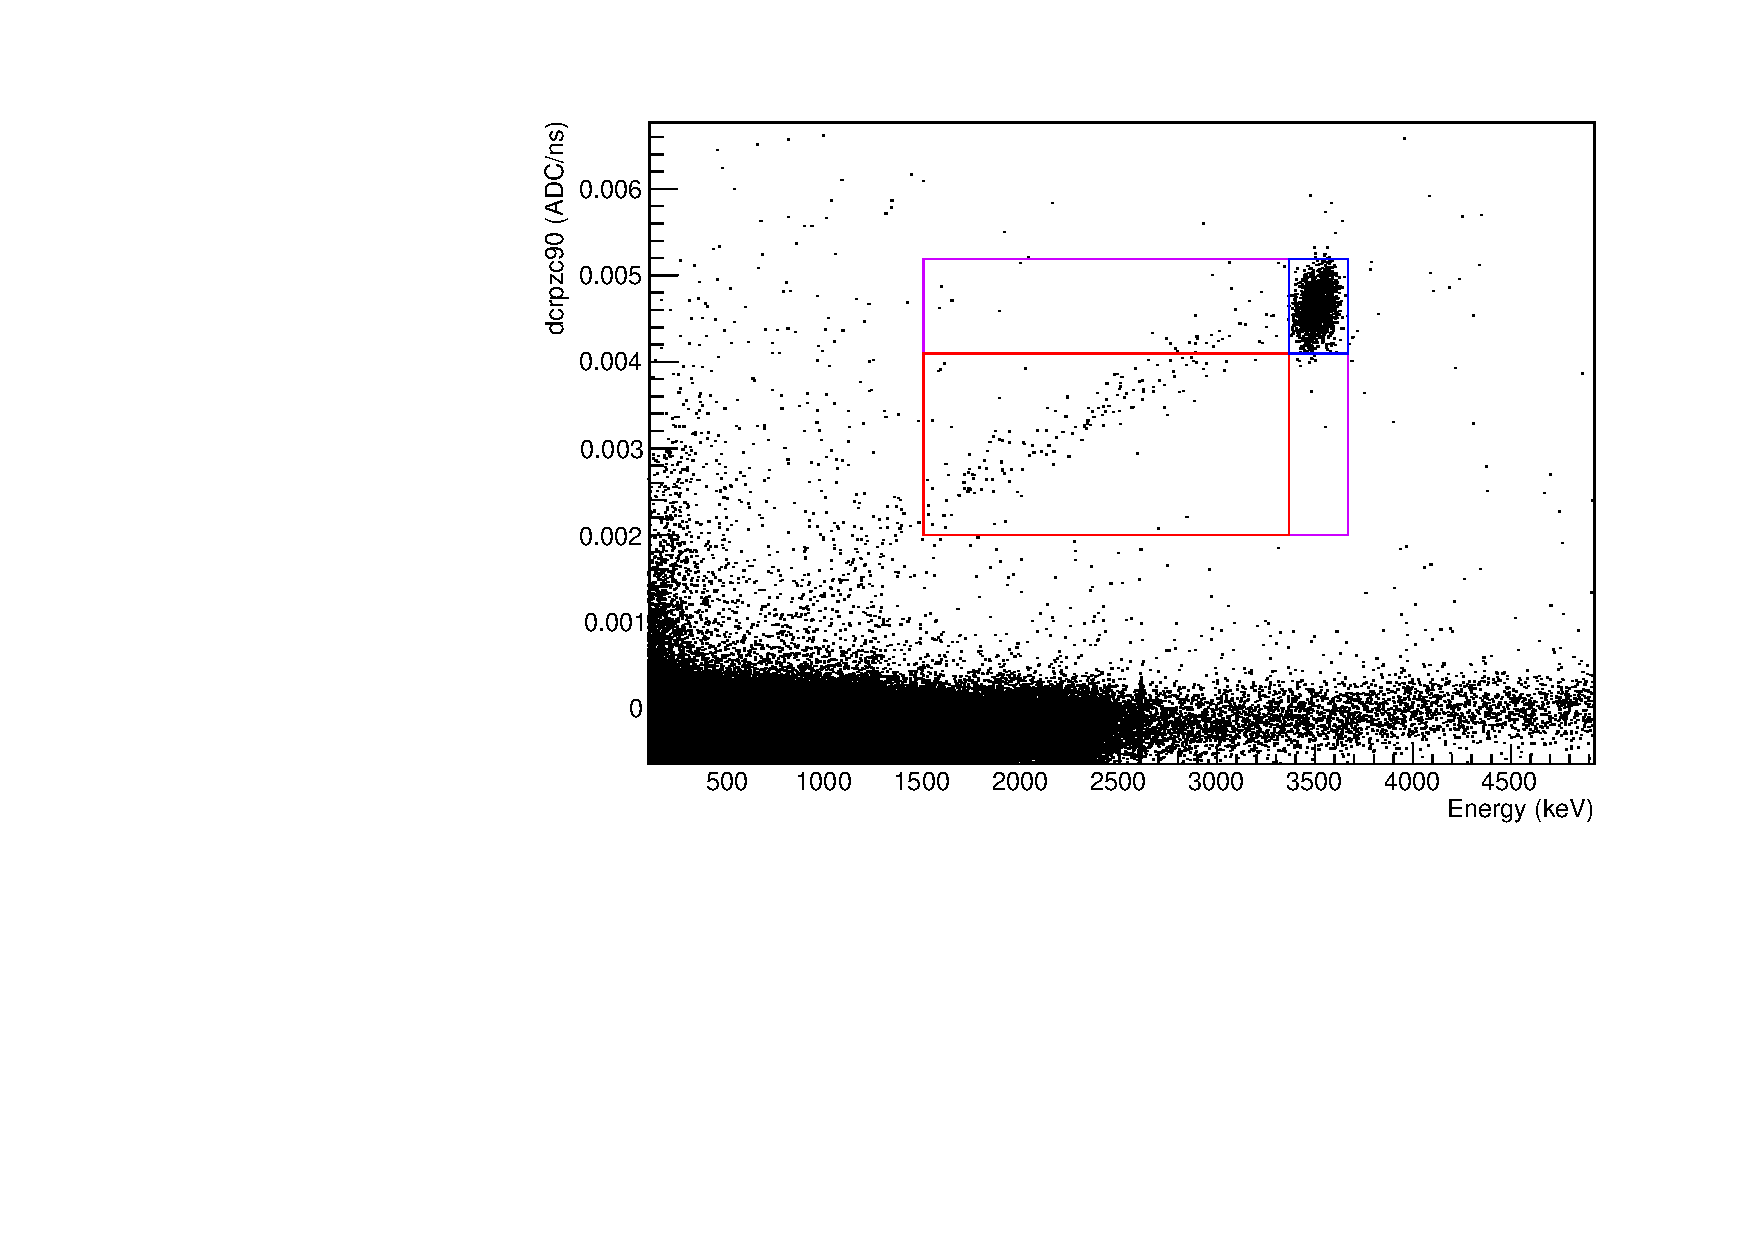
\includegraphics[width=1.0\columnwidth]{figs/outlier_events_260_0.png}
 \caption{A plot of all single-site events in a data set taken at $r=9$\,mm, in {\tt dcrpzc90} vs. energy. The blue box shows the region that lies within $5\sigma$ of the energy and DCR peaks, and the red box indicates some of the events that are outliers from both peaks. Events that are in the violet box but not in the red or blue boxes are outliers in either the energy or DCR peaks. The red-outlined region shows a clear excess of events over a source-free data set. 8.2\% of the events in the violet box (including the red and blue-boxed regions) are outliers from both peaks; 89.2\% fall within the $5\sigma$ windows of both the energy and DCR peaks.} 
 \label{fig:outliers}
\end{figure}


\subsubsection{Radial Dependence of DCR}
The azimuthal dependence (or, we believe, the instability, see below) of the DCR parameters makes it difficult to draw definitive conclusions about their radial dependence. This is particularly the case at large radii ($r>12$\,mm). In positive-radius scanning positions, {\tt dcrpzc90} falls with increasing radius, at a rate of -4.8E-5$\pm$1.2E-5\,ADC/ns/mm, found using a linear fit to all data sets in this position range. In negative-radius scanning positions, {\tt dcrpzc90} instead rises with increasing radius, at a rate of 2.8E-5$\pm$3E-6\,ADC/ns/mm. 

Compared to this, the radial dependence of the DCR parameters at positions with $r<12$\,mm is dramatic, and occurs with similar functional form in both the positive- and negative-radius scans, as seen in Figs. ~\ref{fig:DCRfit_rMag} and ~\ref{fig:dcrNormFit_rMag}. Unfortunately, the source beam is obstructed at small positive-radii positions, so the similarity of the results cannot be tested directly for all radii. 

Over the range that can be scanned, though, the positive-radius positions show a fall {\tt dcrpzc90} rise with increasing radius with a rate of 1.4E-4$\pm$3E-5\,ADC/ns/mm, and the negative-radius positions show an increase with the rate of 3.2E-4$\pm$2E-5\,ADC/ns/mm. If, instead of using all negative-radius data sets, we use only those for which a positive-radius equivalent exists, we derive a rate of change for the {\tt dcrpzc90} value of 1.8E-4$\pm$4E-5\,ADC/ns/mm, which agrees with the rate found at positive-radius positions to within the uncertainty of the fit. 

Most importantly, we find that at incidence positions very close to the point-contact ($r<6$\,mm), the DCR parameters cannot be used to reliably identify alpha events while retaining high bulk-event efficiency. Alphas incident on the point-contact itself are completely indistinguishable by their DCR parameters.   

\subsubsection{Stability of the DCR Value}
The apparent azimuthal dependence of the DCR value is thought, rather, to be a problem of instability in the process by which delayed charge is collected. In studies of the stability, data sets with $|r|<12$\,mm are excluded; based on the observations of the radial dependence of DCR (above), it appears that the changes in DCR at these positions are unaffected by the azimuthal effect or instability, whatever its source. 

The leading candidate for the cause of the shift in the DCR parameters is charging of the detector surface by the alpha particles themselves, and the resulting interactions in the detector surface. Passivated surface charge build-up over time has been observed in other PPC detectors (citation?), and our own measurements of the observed energy indicate that significant charge is being lost on or near the surface. Direct measurement of the leakage current in the detector after the alpha scans were completed showed that it was an order of magnitude higher than at the start of scanning, further supporting this theory. 

Plotting {\tt dcrpzc90} in each data set with respect to the data set order (which corresponds, almost exactly, to days of run time), as in Fig.~\ref{fig:DCRvT}, shows a pattern in which the DCR parameter values rise over the time during which the source is incident on the passivated surface, ``resetting" to lower values after the source beam is removed from the surface for some time. Furthermore, the rate at which the DCR value increases appears to be correlated with the observed alpha rate, as would be expected if surface charge build-up were the cause of the change. 

Additional evidence for this theory is provided by the changes in DCR values in the positions that were repeated non-consecutively, with several days of scanning of other positions occurring between the two scans at that location. This was done for 3 positions, at $r= $  -9, -7.5, and 30\,mm. In all three cases, shown in Fig.~\ref{fig:DCR_repeated}, the second measurement shows a higher DCR value than the first measurement.  

\begin{figure}[]
 \centering
 \includegraphics[width=1.0\columnwidth]{figs/dcrpzc90fit_mu_overTime_rOver12_wRate.png}
 \caption{The {\tt dcrpzc90} mean value of the alpha peak, as a function of data set order. One data set corresponds, almost exactly, to one day of run time. The hashed boxes indicates stretches of time during which the alpha source was not incident on the detector surface. The color scale indicates the alpha event rate, in events/hr.} 
 \label{fig:DCRvT}
\end{figure}

\begin{figure}[]
 \centering
 \includegraphics[width=1.0\columnwidth]{figs/dcrpzc90_repeatedDS.png}
 \caption{The {\tt dcrpzc90} mean value of the alpha peak as a function of data set order for the non-consecutively repeated measurements. The point shapes indicate the position of the source (circles, squares, and triangles correspond to runs with $r=$ -9, -7, and 30\,mm, respectively), and colors indicate the run order (blue is the first data set taken at that position, red is the second). One data set corresponds, almost exactly, to one day of run time. The hashed boxes indicates stretches of time during which the alpha source was not incident on the detector surface.} 
 \label{fig:DCR_repeated}
\end{figure}



\subsection{A/E and DCR} 
\subsubsection{A/E of Alpha Events}
As expected from the calculated drift paths of PPC detectors, the rate of the initial rise of pulses strongly depends on the event incidence radius, particularly near the passivated surface. The high-A/E peak of events associated with the alpha source was fit using a Gaussian function, and its centroid $\mu_{AE}$ was taken as the characteristic A/E value of the scanning location. Since the precise peak shapes of the A/E distributions are not of interest for this work, we use a simplified fitting model, with only a Gaussian component to identify the peak centroid and width. 

For runs in which the energy of the $\alpha$ peak is well over 2630\,keV ($\abs{r} > 7.5$\,mm), only events with energies between 2630\,keV and 6\,MeV are included. For data sets with $\abs{r} < 7.5$\,mm, where all or some of the alpha peak may fall outside this energy window, events with energies between 1 and 6\,MeV are included. See Fig.~\ref{fig:AE_fits} for sample A/E distributions and fits. 

\begin{figure*}[]
 \centering
 \begin{subfigure}[]{.45\textwidth}
 \includegraphics[width=1.0\columnwidth]{figs/DS10_0_aefit.png}
 \caption{A data set taken at 1 turn ($r = -28.5$\,mm), a total of 24.9\,hrs of runtime, with a cut selecting events with energy between 2630\,keV and 6\,MeV.}
\end{subfigure}
 \begin{subfigure}[]{.45\textwidth}
 \includegraphics[width=1.0\columnwidth]{figs/DS170_0_aefit.png}
  \caption{A data set taken at 17 turns ($r = -4.5$\,mm), a total of 19.1\,hrs of runtime, with a cut selecting events with energy between 1\,MeV and 6\,MeV.} 
\end{subfigure}
\caption{Sample A/E distributions and Gaussian peak fits to alpha events.}
 \label{fig:AE_fits}
\end{figure*}

For most data sets, the peak in A/E is approximately Gaussian in shape. As in the case of energy, the peak becomes non-Gaussian at small radii, where the length scale of significant changes to the drift time of charges becomes small compared to the diameter of the source beam. At these small radii, however, the A/E values are well above those of 99\% of background events. 

Anomalously low values of A/E occur for events incident on the point-contact itself. Though these events have very fast rising edges, they also have a substantial slow electron fraction, which reduces the A/E value. To correctly identify events like these from the shape of their rising edge, a rise-time parameter, measuring time over which the pulse rises from the start of the prompt signal to a given fraction of its total amplitude (for instance, 50\% of the maximum pulse height), would be more appropriate than the A/E parameter used in this analysis. The \MJ\ Collaboration plans to implement such a pulse-shape discriminator, in addition to the {\tt avse} parameter that is currently used to reject multi-site events.

The fit results are displayed in Fig.~\ref{fig:AEfit_mu}. These results indicate that the high-A/E cut applied to give energy and DCR fit results,  as in Sec.~\ref{ssec:E_obs}, is appropriate.

\begin{figure}[]
 \centering
 \includegraphics[width=1.0\columnwidth]{figs/AEvR_wBox.png}
 \caption{The centroids of the alpha peaks in A/E in each data set. The relatively low value of A/E for data sets with $r=-0.75$\,mm occurs because the large (slow) electron component of the signal reduces the A/E value for these events.} 
 \label{fig:AEfit_mu}
\end{figure}

\subsubsection{Complementarity of High-A/E and DCR Cuts}
The distributions of alpha events incident at various radii in the A/E vs. DCR parameter space (see Fig.~\ref{fig:AEvDCR_events}) suggest that the two pulse-shape analyses are highly complementary. This suggests that by using both the A/E and DCR pulse shape discriminators, we should be able to achieve excellent alpha event discrimination with only minimal sacrifice of bulk events. 

\begin{figure*}[]
 \centering
 \begin{subfigure}{.65\textwidth}
 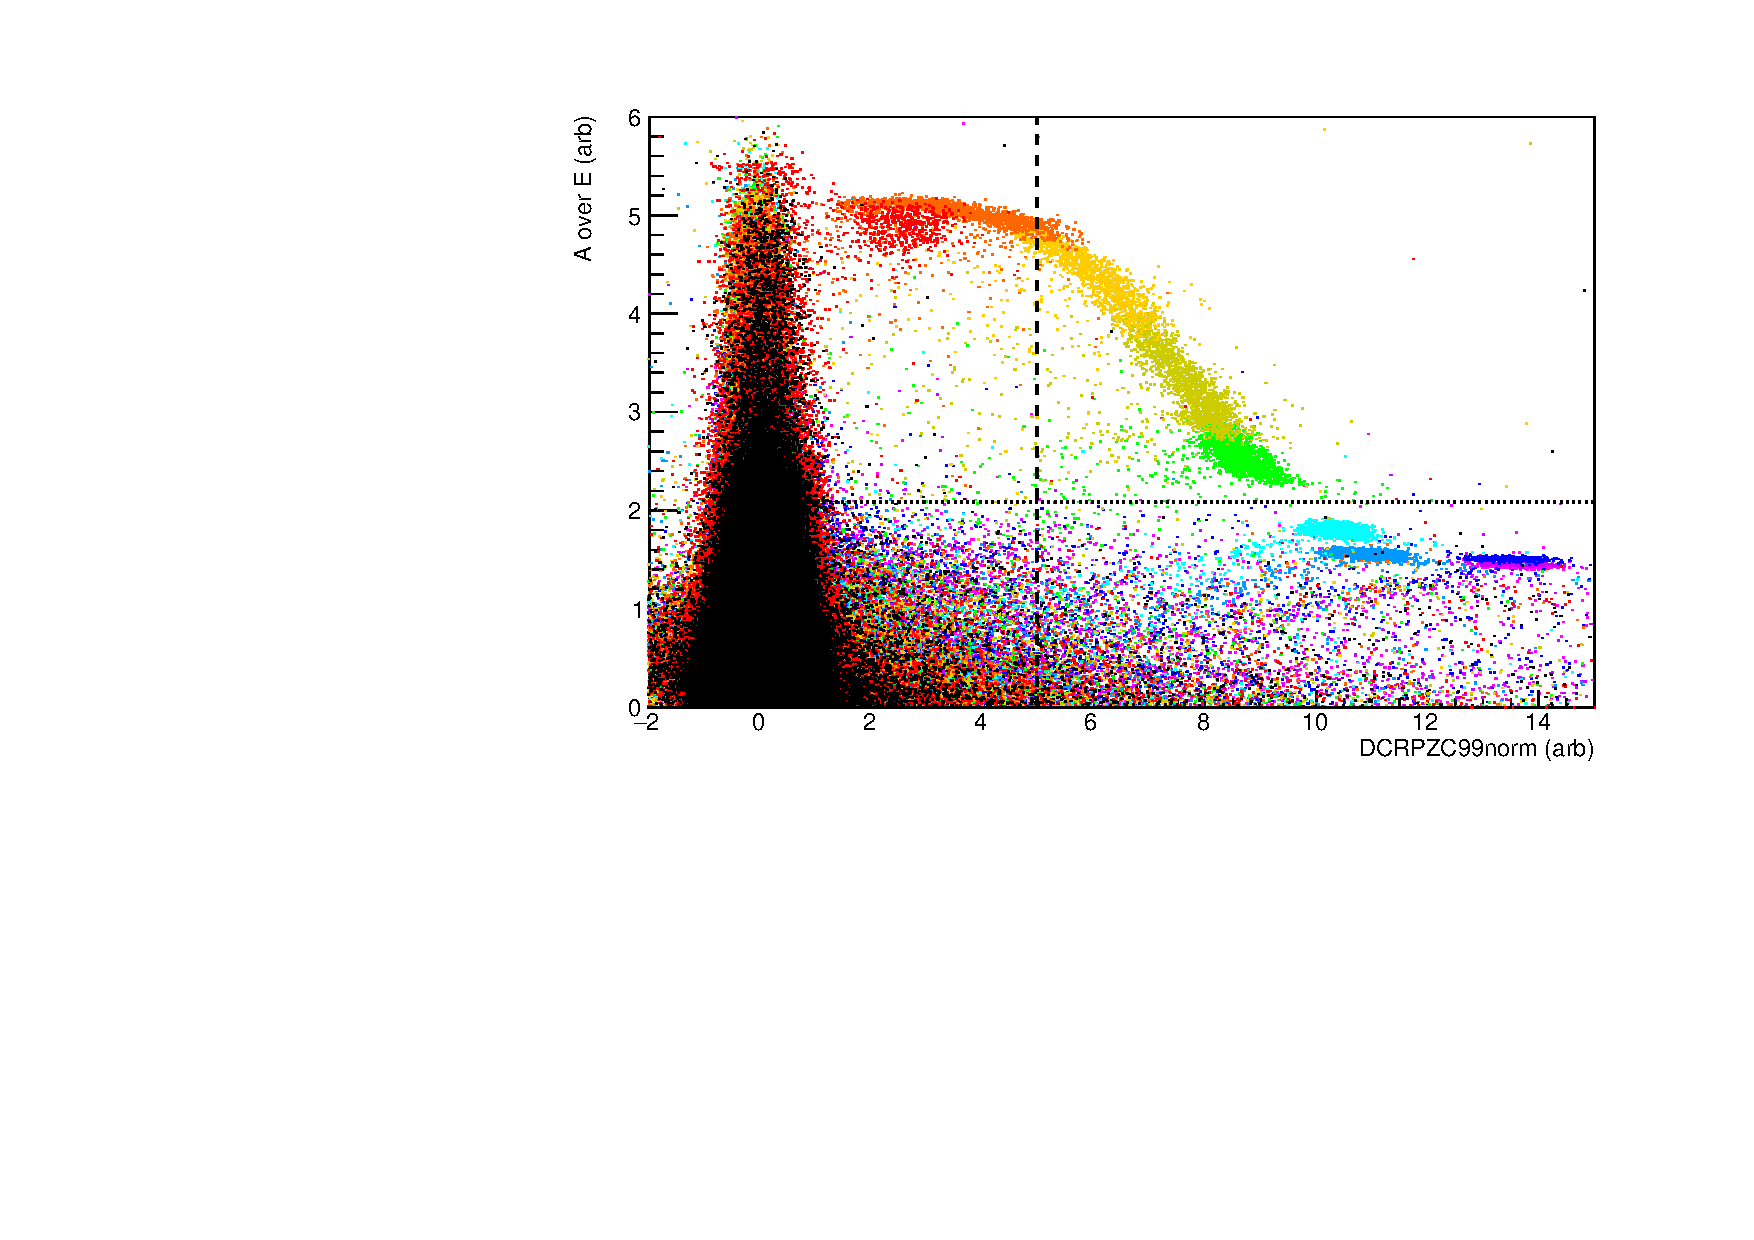
\includegraphics[width=1.\columnwidth]{figs/AEvDCRPZCnorm.png}
 \end{subfigure}
 \begin{subfigure}{.34\textwidth}
  \includegraphics[width=1.\columnwidth]{figs/AEvDCR_plot_legend.png}
   \end{subfigure}
 \caption{The A/E vs. normalized DCR distribution for all single-site events with energies between 100\,keV and 10\,MeV, at varying scanning radii. The points in black are from a data set without the alpha source incident on the detector surface, and the scan data sets are shown in rainbow order, with red representing the smallest-radius scan. 99\% of calibration events with energies between 1000 and 2630\,keV fall below an A/E value of 1, and 99\% of calibration events with energies between 1000 and 2380\,keV fall below a {\tt dcrpzc99norm} value of 1.} 
 \label{fig:AEvDCR_events}
\end{figure*}

Examining the fit results to the DCR and A/E peaks supports this conclusion. The $5\sigma$ windows around each alpha peak should include 99\% of the events, assuming normally distributed values; by using an equivalent normalization for the A/E and DCR values, we can compare them directly, as in Fig.~\ref{fig:AEandDCR}. The y-axis in this figure indicates the alpha events' separation from bulk events-- 99\% of bulk events fall below 1, whether the relevant discrimination parameter is A/E or DCR. Also indicated are the 99.9\% acceptance points in each parameter, which occur at different values for A/E and DCR, indicating that the DCR distribution is more heavily-tailed than the A/E distribution. 

\begin{figure*}[]
 \centering
 \includegraphics[width=1.\textwidth]{figs/AEandDCR_noThree.png}
 \caption{The $5\sigma$ window containing the A/E and DCR alpha peak positions at each position, normalized to 99\% bulk acceptance of both cuts. The red points and magenta boxes indicate the centroids and $\pm 2.5\sigma$ values of the peaks in {\tt dcrpzc99norm}, and the green points and blue boxes indicate the same in {\tt aenorm}. The red dotted line and cyan dotted-dashed line are the 99.9\% acceptance points in DCR and A/E, respectively. The black dashed line indicates the 99\% acceptance point in both parameters.} 
 \label{fig:AEandDCR}
\end{figure*}

For each position measured, we find that either or both of the DCR and A/E discriminator parameters are well above the 99.9\% acceptance line for that parameter. This indicates that by applying 99.9\% bulk-acceptance cuts in both parameters, we can effectively eliminate alpha events occurring anywhere on the passivated surface. Ergo, total alpha event rejection with only 0.2\% sacrifice of bulk events should be possible in PPC detectors.

Another advantage of this method of alpha removal is that it is equally effective at all energies of the alpha events, save for the requirement that the energy of the event be high enough that the DCR signal (of approximately 2-3\% of the prompt event energy, see above) is detectable. This is the case for all events that could fall in the \nonubb\ ROI. Therefore, this purely pulse-shape-based method is as effective for energy-degraded alpha events as it is for undegraded events originating from alpha contamination on the surface itself.

The only exception to this highly efficient alpha event removal occurs for events directly incident on the point-contact itself, at the smallest-radius position. Given that these events do not experience charge trapping, their energies are much higher than that of the \nonubb\ region-of-interest, so they are not a particularly problematic background. If alpha energy is degraded before reaching the point-contact, though, they could have any energy below the full energy of the alpha peak. As discussed above, these events would be effectively tagged with high efficiency if a rise-time parameter were substituted for the A/E parameter, as is planned in the \MJ\ \DEM\ analysis. 

Fig.~\ref{fig:AEandDCR} also shows that at positions with $r<= 6$\,mm, the A/E-based rejection of alpha events dominates in effectiveness, and that below $r=9$\,mm, an 99.9\%-acceptance cut in A/E suffices to tag all alpha events. This is why the previous study of alpha backgrounds in a PPC detector \cite{Agostini_thesis}, found no need for an additional pulse-shape discriminator beyond A/E, though an asymmetry parameter, which identifies slowly-released charge like our DCR parameter, was studied \cite{TUBEdoc?}. BEGe-type detectors, like the one measured in that work, have the entirety of their passivated surface lying within $r=9$\,mm, so the use of the DCR discriminator would not measurably improve their background rejection capabilities. 

The DCR discriminator is needed, though, in ORTEC-type detectors, which have a passivated surface along the entire bottom plane of the detector. In this detector design, which is that of the detector measured in this work, and used for all of the \MJ\ \DEM 's enriched detectors, the DCR discriminator is a powerful way to reject alpha events occurring far from the point-contact, where A/E is relatively insensitive. 

\subsection{Alpha-Identification Efficiency using DCR Techniques}
Given that the DCR pulse-shape discrimination technique is less effective than the A/E technique at $r<=6$\,mm, we focus our attention on evaluating the alpha-rejection efficiency of the various DCR parameters at scanning positions with $r>6$\,mm. 

To calculate an alpha-rejection fraction, we must first find the predicated number of background events in the alpha peak region of the data set, with no DCR cut applied. We use both the right-hand sideband in the data set and the spectral shape in the sideband and peak regions, measured in a source-free run, to find the expected number of background events. See Fig.~\ref{fig:eff_regions} for sample spectra and energy regions. 

\begin{figure*}[]
 \centering
 \includegraphics[width=1.\textwidth]{figs/eff_peakRegions.png}
 \caption{Energy spectra for a source scan data set with $r=9$\,mm {\it (left)} and a background data set {\it (right)}. The energy windows indicated are the $5\sigma$ peak region, in red, and the 500\,keV right-hand sideband, in blue. $n_{s, pk}$ is the sum of all events in the red solid-lined box and $n_{s, rh}$ is the sum of all the events in the blue solid-lined box. $n_{b, pk}$ and $n_{b, rh}$ are the sum of events in the red and blue dashed-line boxes, respectively.} 
 \label{fig:eff_regions}
\end{figure*}

Below, the background data set is referred to by the subscript {\it b} and the alpha source scanning data set by the subscript {\it s}. The peak region is taken to be a $5\sigma_E$ window around the centroid of the alpha-energy Gaussian, and the sideband region is the 500\,keV region with minimum energy of $\mu_E+5\sigma_E$. Only a right-hand sideband is used, to avoid effects from the energy-degraded alpha events described in Sec.~\ref{sssec:outliers}. The peak region is referred to by the subscript {\it pk}, and the sideband region by the subscript {\it rh}.

The following algorithm is repeated for each alpha scan data set for which we would like to calculate the efficiency:
\begin{itemize}
\item The expected spectral shape of the background events is calculated from a background run. To do this, the number of events in the peak region, $n_{b, pk}$, and the number of events in the right-hand sideband region, $n_{b, rh}$ are found. Each event total is divided by the width of its energy window. Their ratio is the number of events per keV expected in the peak region, given some number of events per keV in the sideband region.
\item The number of events in the right-hand sideband of the source scan data set, $n_{s, rh}$ is found. It is normalized by the width of the sideband energy window, and then multiplied by the width of the peak energy window and the spectral shape ratio to give the number of background events per hour expected in the peak region. 
\item This value is subtracted from the measured number of peak-region events in the alpha source scan data set, $n_{s, pk}$ to give the projected number of alpha events, $n_{\alpha}$. I.e., 
$$ n_{\alpha} =  n_{s, pk}-n_{s, rh}\frac{n_{b, pk}}{n_{b, rh}}\frac{5\sigma_E}{500\,keV} $$
\item The above steps are repeated after the DCR cut is applied to both the source and background runs to find the expected number of background events in the peak region of the source scan data set that would be removed by the cut. This value is subtracted from the total number of events cut in the peak region of the source data set to give the projected number of alpha events removed by the cut, $m_\alpha$. I.e.,
 $$ m_{\alpha} =  m_{s, pk}-m_{s, rh}\frac{m_{b, pk}}{m_{b, rh}}\frac{5\sigma_E}{500\,keV} $$
 where the $m_{i, j}$ are equivalent to the $n_{i, j}$ above, but measured after the DCR cut is applied. 
\item The ratio $\frac{m_\alpha}{n_\alpha}$ is the alpha rejection efficiency in the source-scan data set. 
\end{itemize}

A derivation of the formula by which the uncertainties for these efficiencies are calculated is given in Appendix FIXME. 

At positions with radii below 6\,mm for which the source is incident on the passivated surface, the alpha peak appears in a region of the energy spectrum that is dominated by gamma background events from environmental radioactivity and the materials of the cryostat itself. The alpha event rate is low, and these backgrounds are both high and highly variable. An additional complication comes from the broad energy distribution of the alpha events at these positions, as discussed in Sec.~\ref{ssec:E_obs}; to find an expected alpha event rate, we must understand the spectral shape over the entire range of relevant energies with high accuracy. 

This implies that our approach of normalizing the background spectra to one another is of limited utility.  The resulting uncertainties from the estimate of the backgrounds dominate our expected alpha event rate. Without an accurate calculation of the expected number of alpha events, we cannot accurately cite a rejection fraction for the events. Therefore, measurements at these radii are not included in the average efficiency values for each DCR parameter. 

Events incident on the point-contact itself are not expected to exhibit slow charge release, and are therefore expected to be relatively unaffected by the DCR cut. Data sets with the source beam incident on the point-contact are therefore also excluded from the average efficiency calculations. 

The rejection efficiencies are calculated for each data set using the {\tt dcr90}, {\tt mjddcr90}, and {\tt dcrpzc90}, and {\tt dcrpzc99norm} parameters. The first three of these are set to retain 90\% of single-site calibration events, and the final cut is set to retain 99\% of calibration events. The results for each data set are shown in Fig.~\ref{fig:eff_allR}, and the average rejection efficiency values for each parameter are given in Table~\ref{tab:avgEff}. 

The errors for the efficiency of each data set are large, due to the low alpha rate. They are particularly large at positions with large-magnitude negative radii, where the source beam is partially obscured. 

Averaging the efficiency at all scanning positions, however, reduces the error sufficiently to show that the rejection efficiencies of the various DCR parameters, save for {\tt dcrpzc99norm}, are consistent with 99\%. This implies that 1\% of alpha events with the full expected energy (indicating that significant charge trapping has occurred) are not measurably re-releasing that charge on the time scale of digitization. The higher average efficiency of the normalized DCR parameter ({\tt dcrpzc99norm}), which is consistent with 100\%, suggests that the culprit may be varying noise in the system, which is corrected for by the use of this parameter. This is unsurprising, given the high noise (and particularly the high and varying levels of microphonic noise, due to the vacuum pump operation) in the TUBE scanning setup. 

\begin{figure*}[]
 \centering
 \begin{subfigure}{.45\textwidth}
 \includegraphics[width=1.\textwidth]{figs/dcrpzc_eff.png}
 \caption{The DCR parameters that employ event-by-event pole-zero correction. Values for {\tt dcrpzc90} are in red, and those for {\tt dcrpzc99norm} are in blue.} 
 \end{subfigure}
  \begin{subfigure}{.45\textwidth}
 \includegraphics[width=1.\textwidth]{figs/dcr_eff.png}
 \caption{The DCR parameters that employ the linear projection method of pole-zero correction. Values for {\tt dcr90} are in red, and those for {\tt mjddcr90} are in blue.} 
 \end{subfigure}
 \caption{The alpha rejection efficiency of each DCR parameter, calculated for each data set with a source beam incidence position with $r>6$\,mm.}
 \label{fig:eff_allR}
\end{figure*}

\begin{table}[]
\begin{center}
\begin{tabular}{l r r}
DCR Param. & ~~$\varepsilon$ (\%), $|r|>6$\,mm \\  \hline
{\tt dcr90} & 99.2$\pm$0.5  \\
{\tt dcrpzc90} & 98.9$\pm$0.5  \\
{\tt mjddcr90} & 99.1$\pm$0.5  \\
{\tt dcrpzc99norm} &  99.7$\pm$0.4 \\
\end{tabular}
\caption{Average alpha rejection efficiencies for all evaluated DCR parameters.} \label{tab:avgEff}
\end{center}
\end{table}


\section{Comparison to Models of Surface-Charge Collection}
\subsection{Surface Drift of Electrons}
\subsection{Surface Drift of Electrons and Holes}
\subsection{Passivated-Surface Trapping of Holes}

\section{Implications for the \MJ\ \DEM\ }
\subsection{Overall DCR Efficiency}
\subsubsection{Uniform-distribution Model}
\subsubsection{Point-contact Contamination Model}

\subsection{Projections of $\alpha$ Contamination in the \MJ\ \DEM\ Spectrum}

\section{Future Work}



%%%%%% Any additional considerations for a publication %%%%%%
\section{Journal Thoughts}



\bibliographystyle{plainnat}
\bibliography{unidoc_temp}




\end{document}
